\chapter{Phân tích và thiết kế hệ thống}
\label{chap:phantich}

\section{Phân tích đối tượng người dùng}
\label{sec:doituongnguoidung}

\subsection*{a) Nông dân / hợp tác xã (HTX)}
\begin{itemize}
    \item \textbf{Nhu cầu:} bán được sản lượng thu hoạch với giá công bằng hơn kênh thương lái; tiếp cận trực tiếp khách hàng B2B (nhà hàng, siêu thị) để có đơn hàng ổn định theo hợp đồng; xây dựng thương hiệu/uy tín cá nhân qua lịch sử đánh giá và chứng nhận.
    \item \textbf{Khó khăn:} hạn chế kỹ năng số và thiết bị (điện thoại thông minh, internet ổn định ở vùng sâu vùng xa); thiếu năng lực tự chụp ảnh/ghi nhật ký canh tác đúng chuẩn; e ngại công nghệ và lo sợ bị nền tảng ``thu phí thay thương lái'' mà không mang lại giá tốt hơn thực chất.
    \item \textbf{Vai trò hệ thống (RBAC):} \texttt{seller} --- được gán sau khi hoàn tất xác thực (mục~\ref{sec:luongtiepcan}).
\end{itemize}

\subsection*{b) Người tiêu dùng cá nhân}
\begin{itemize}
    \item \textbf{Nhu cầu:} mua nông sản tươi, an toàn, có thể tra cứu nguồn gốc rõ ràng, giá cả hợp lý, giao hàng nhanh và đúng chất lượng như hình ảnh/mô tả.
    \item \textbf{Khó khăn:} khó phân biệt sản phẩm ``sạch'' thật với sản phẩm gắn mác marketing (do bất cân xứng thông tin --- mục~\ref{subsec:reputation}); lo ngại hàng tươi bị hư hỏng trong vận chuyển; thói quen mua sắm tại chợ/siêu thị truyền thống vẫn phổ biến, đòi hỏi sàn TMĐT phải tạo được lòng tin đủ lớn để thay đổi hành vi.
    \item \textbf{Vai trò hệ thống (RBAC):} \texttt{buyer\_retail} --- được gán ngay sau xác thực OTP (mục~\ref{sec:luongtiepcan}).
\end{itemize}

\subsection*{c) Doanh nghiệp thu mua (nhà hàng, siêu thị, nhà phân phối)}
\begin{itemize}
    \item \textbf{Nhu cầu:} nguồn cung ổn định về số lượng/chất lượng theo tiêu chuẩn (VietGAP/GlobalGAP tùy nội địa hay xuất khẩu); đặt hàng theo hợp đồng/lịch giao định kỳ; cơ chế giá theo sản lượng (giá bậc) và công nợ/thanh toán linh hoạt.
    \item \textbf{Khó khăn:} khó tìm và xác minh nhiều nhà cung cấp nhỏ lẻ phân tán; rủi ro đứt gãy cung ứng khi mất mùa hoặc nhà cung cấp không đáp ứng MOQ; thiếu công cụ quản lý hợp đồng/hóa đơn tập trung khi làm việc với nhiều nông dân/HTX riêng lẻ.
    \item \textbf{Vai trò hệ thống (RBAC):} \texttt{buyer\_wholesale} --- được gán sau khi đội ngũ kinh doanh xác minh hồ sơ doanh nghiệp (mục~\ref{sec:luongtiepcan}).
\end{itemize}

\subsection*{d) Quản trị viên hệ thống}
\begin{itemize}
    \item \textbf{Nhu cầu:} công cụ kiểm duyệt hiệu quả (nhà bán, sản phẩm, chứng nhận); công cụ giám sát và xử lý vi phạm (hàng giả nhãn, gian lận chứng nhận, khiếu nại gian dối); báo cáo thống kê hỗ trợ ra quyết định vận hành.
    \item \textbf{Khó khăn:} khối lượng kiểm duyệt lớn khi số nhà bán tăng nhanh; khó xác minh tính xác thực chứng nhận VietGAP/GlobalGAP nếu không có API kết nối cơ quan cấp chứng nhận; cân bằng giữa kiểm duyệt chặt (đảm bảo chất lượng) và tốc độ duyệt (không làm nản lòng nhà bán mới).
    \item \textbf{Vai trò hệ thống (RBAC):} \texttt{admin} --- được cấp nội bộ, không qua kênh đăng ký công khai (mục~\ref{sec:luongtiepcan}).
\end{itemize}

\section{Luồng tiếp cận và tham gia hệ thống}
\label{sec:luongtiepcan}

Mục này làm rõ cách mỗi nhóm người dùng ở mục~\ref{sec:doituongnguoidung} biết đến, liên hệ và được cấp quyền tham gia Farmery — trước khi đi vào chi tiết từng quy trình nghiệp vụ ở mục~\ref{sec:quytrinhnghiepvu}.

\subsection*{Nhà bán (nông dân/HTX)}
\begin{itemize}
    \item \textbf{Kênh tiếp cận:} giới thiệu qua hội nông dân/HTX địa phương, chương trình OCOP (mục~\ref{chap:coso}), hoặc tự đăng ký trực tiếp trên web/app Farmery.
    \item \textbf{Liên hệ hỗ trợ:} đội ngũ hỗ trợ vùng (hotline/Zalo OA) hướng dẫn nhập thông tin trang trại và ghi nhật ký canh tác cho nhóm ít rành công nghệ.
    \item \textbf{Thủ tục:} quy trình đăng ký, xác thực OTP và kiểm duyệt chứng nhận — chi tiết đầy đủ tại mục~\ref{sec:quytrinhnghiepvu} (Đăng ký và xác thực nhà bán).
    \item \textbf{Kết quả:} tài khoản chuyển trạng thái ``Đã xác thực'', được gán vai trò \texttt{seller}, có thể đăng bán lẻ và/hoặc công bố bảng giá bán sỉ.
\end{itemize}

\subsection*{Người mua lẻ (người tiêu dùng cá nhân)}
\begin{itemize}
    \item \textbf{Kênh tiếp cận:} tự đăng ký trên web/app qua kênh quảng bá số (mạng xã hội, SEO) hoặc giới thiệu từ cộng đồng quan tâm nông sản sạch.
    \item \textbf{Liên hệ hỗ trợ:} kênh CSKH chung (chat/hotline) cho các thắc mắc về đơn hàng, đổi trả.
    \item \textbf{Thủ tục:} đăng ký số điện thoại hoặc email, xác thực OTP — không yêu cầu xác minh giấy tờ, có thể mua ngay sau khi xác thực.
    \item \textbf{Kết quả:} tài khoản được gán vai trò \texttt{buyer\_retail}, truy cập ngay quy trình bán lẻ (mục~\ref{sec:quytrinhnghiepvu}).
\end{itemize}

\subsection*{Người mua sỉ (doanh nghiệp thu mua)}
\begin{itemize}
    \item \textbf{Kênh tiếp cận:} đăng ký tài khoản doanh nghiệp qua form riêng trên nền tảng, hoặc liên hệ trực tiếp đội ngũ kinh doanh (account manager) của Farmery để được tư vấn.
    \item \textbf{Liên hệ hỗ trợ:} account manager phụ trách khu vực/ngành hàng, hỗ trợ thiết lập hạn mức công nợ phù hợp quy mô doanh nghiệp.
    \item \textbf{Thủ tục:} khai báo mã số thuế/giấy phép kinh doanh, đội ngũ Farmery xác minh hồ sơ trước khi cấp quyền xem bảng giá sỉ và gửi RFQ — thời gian xử lý dài hơn nhóm mua lẻ do cần thẩm định.
    \item \textbf{Kết quả:} tài khoản được gán vai trò \texttt{buyer\_wholesale}, truy cập quy trình bán sỉ (mục~\ref{sec:quytrinhnghiepvu}).
\end{itemize}

\subsection*{Quản trị viên}
\begin{itemize}
    \item \textbf{Kênh tiếp cận:} không có kênh đăng ký công khai — tài khoản được ban quản trị/Chủ nhiệm Bộ môn hệ thống cấp phát nội bộ.
    \item \textbf{Thủ tục:} gán vai trò \texttt{admin} (hoặc vai trò quản trị chuyên biệt hơn khi hệ thống mở rộng — mục~\ref{chap:coso}) theo nguyên tắc đặc quyền tối thiểu.
\end{itemize}

Khi hoàn tất thủ tục tham gia ở trên, mọi tài khoản đều chịu sự ràng buộc của Điều khoản dịch vụ (Phụ lục D) --- quy định đầy đủ quyền, nghĩa vụ, phí và cơ chế xử lý tranh chấp giữa các bên.

\section{Phân tích mô hình kinh doanh}
\label{sec:businessmodelcanvas}

Dựa trên khung Business Model Canvas (mục~\ref{subsec:businessmodel}), Hình~\ref{fig:bmc} trình bày mô hình kinh doanh cụ thể của Farmery.

\begin{figure}[H]
\centering
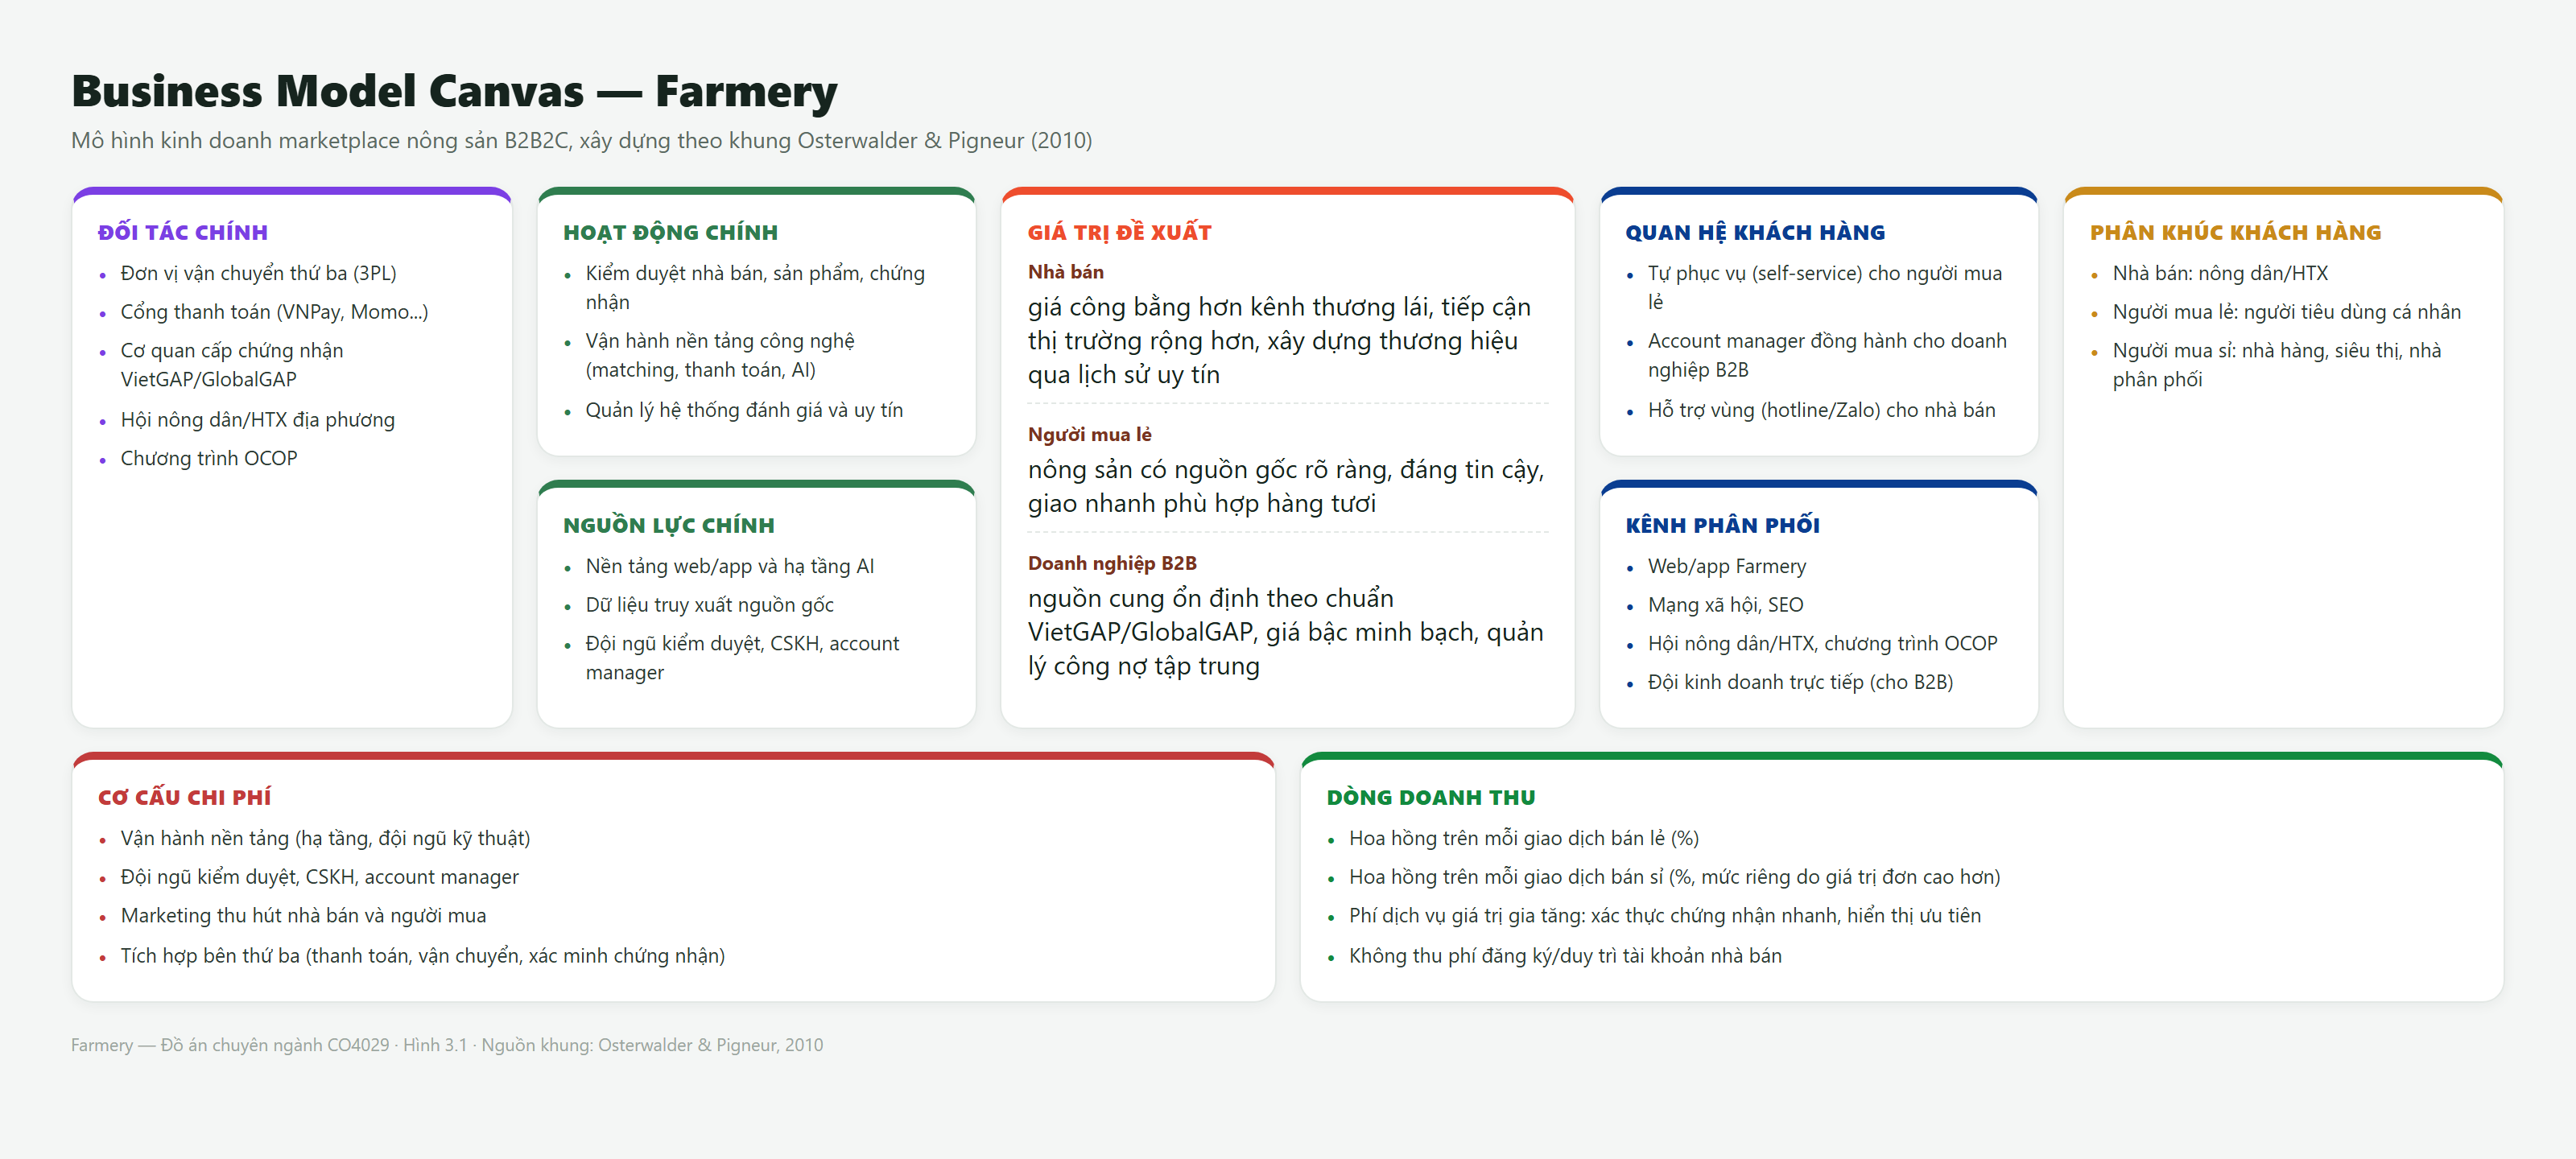
\includegraphics[width=\textwidth]{image/comparison/business-model-canvas.png}
\caption{Business Model Canvas của Farmery}
\label{fig:bmc}
\end{figure}

Dòng doanh thu chính là phí hoa hồng trên mỗi giao dịch thành công, tách theo hai mức cho bán lẻ và bán sỉ (mục~\ref{sec:quytrinhnghiepvu}) do biên lợi nhuận và giá trị đơn hàng trung bình của hai kênh khác nhau đáng kể; ngoài ra còn có phí dịch vụ giá trị gia tăng (xác thực chứng nhận nhanh, hiển thị ưu tiên cho nhà bán đạt ngưỡng uy tín cao --- mục~\ref{subsec:danhgianghiepvu}). Nền tảng chủ động không thu phí đăng ký hoặc phí duy trì tài khoản đối với nhà bán, nhằm giảm rào cản gia nhập cho nhóm nông dân/HTX vốn đã hạn chế về nguồn lực (mục~\ref{sec:doituongnguoidung}) --- chi tiết mức phí cụ thể và các điều khoản liên quan được quy định tại Phụ lục D (Điều khoản dịch vụ).

\section{Yêu cầu chức năng}
\label{sec:yeucauchucnang}

Dựa trên phân tích đối tượng người dùng (mục~\ref{sec:doituongnguoidung}) và
quy trình nghiệp vụ (mục~\ref{sec:quytrinhnghiepvu}), hệ thống cần đáp ứng các
nhóm yêu cầu chức năng sau. Các mã FRx.x dùng để đối chiếu 1--1 với use case
tại mục~\ref{sec:sddchitiet} và phần hiện thực ở Chương~4.

\subsection{FR1: Quản lý tài khoản \& phân quyền}
\begin{itemize}
    \item \textbf{FR1.1:} Đăng ký/đăng nhập theo vai trò riêng biệt: nông
    dân/HTX, người tiêu dùng, doanh nghiệp thu mua (B2B), quản trị viên; hỗ
    trợ đăng nhập bằng Email, số điện thoại hoặc tài khoản mạng xã hội
    (OAuth 2.0).
    \item \textbf{FR1.2:} Xác thực tài khoản qua OTP (đăng ký, khôi phục mật
    khẩu, các thao tác nhạy cảm).
    \item \textbf{FR1.3:} Đăng ký tài khoản doanh nghiệp thu mua (B2B) kèm
    xác thực Giấy phép kinh doanh (GPKD) và Mã số thuế (MST).
    \item \textbf{FR1.4:} Phân quyền nội bộ cho tài khoản doanh nghiệp theo
    mô hình RBAC (Chủ tài khoản, Người mua hàng, Kế toán, Người xem) --- liên
    hệ mục~\ref{chap:coso}.
    \item \textbf{FR1.5:} Quy trình xác minh danh tính người bán (eKYC) đối
    với nông dân/HTX trước khi kích hoạt quyền đăng bán.
    \item \textbf{FR1.6:} Quản lý sổ địa chỉ giao/nhận hàng (nhiều địa chỉ,
    gán nhãn, chọn địa chỉ mặc định).
\end{itemize}

\subsection{FR2: Quản lý hồ sơ nông dân/HTX \& gian hàng}
\begin{itemize}
    \item \textbf{FR2.1:} Thiết lập, cập nhật hồ sơ gian hàng (tên, logo,
    mô tả, thông tin vùng trồng/khu vực canh tác).
    \item \textbf{FR2.2:} Báo cáo thống kê cơ bản cho người bán: doanh thu,
    số đơn hàng, sản phẩm bán chạy theo mốc thời gian.
    \item \textbf{FR2.3:} Quản lý tồn kho theo lô hàng (Batch/Lot), gồm số
    lượng nhập/xuất và tồn hiện tại.
\end{itemize}

\subsection{FR3: Quản lý chứng nhận chất lượng}
\begin{itemize}
    \item \textbf{FR3.1:} Tải lên chứng nhận VietGAP/GlobalGAP (và tương tự
    như OCOP, HACCP nếu có) kèm tệp minh chứng.
    \item \textbf{FR3.2:} Quản trị viên kiểm duyệt, phê duyệt hoặc từ chối
    chứng nhận trước khi hiển thị công khai.
    \item \textbf{FR3.3:} Theo dõi hạn hiệu lực chứng nhận, tự động đánh dấu
    hết hạn và nhắc người bán gia hạn (liên hệ FR11.2).
\end{itemize}

\subsection{FR4: Quản lý sản phẩm \& truy xuất nguồn gốc}
\begin{itemize}
    \item \textbf{FR4.1:} Đăng bán sản phẩm kèm hình ảnh, mô tả, đơn vị
    tính (kg, tấn, thùng), giá bán lẻ và bảng giá bán sỉ theo bậc số lượng.
    \item \textbf{FR4.2:} Ghi nhật ký canh tác theo lô (ngày gieo trồng, xử
    lý, thu hoạch) và sinh mã QR truy xuất nguồn gốc gắn với từng lô.
    \item \textbf{FR4.3:} Trừ/khóa tồn kho khi phát sinh giao dịch, tránh
    bán vượt số lượng tồn thực tế.
    \item \textbf{FR4.4:} Phân loại sản phẩm theo danh mục đa cấp chuyên
    ngành nông sản.
    \item \textbf{FR4.5:} Tìm kiếm và lọc nâng cao (khoảng giá, vùng miền,
    loại chứng nhận, đánh giá, tình trạng còn hàng).
\end{itemize}

\subsection{FR5: Giao dịch bán lẻ (B2C)}
\begin{itemize}
    \item \textbf{FR5.1:} Giỏ hàng tổng hợp sản phẩm từ nhiều gian hàng
    trong một phiên mua sắm.
    \item \textbf{FR5.2:} Tự động tách đơn hàng chính thành các đơn con
    theo từng gian hàng tại bước thanh toán.
    \item \textbf{FR5.3:} Áp dụng mã giảm giá (toàn sàn hoặc riêng từng
    gian hàng).
    \item \textbf{FR5.4:} Theo dõi trạng thái từng đơn con độc lập; xử lý
    hủy đơn, đổi trả, hoàn tiền theo từng đơn con.
    \item \textbf{FR5.5:} Đánh giá sản phẩm (điểm số, nhận xét, hình ảnh)
    và đánh giá gian hàng sau khi nhận hàng; người bán có thể phản hồi công
    khai.
\end{itemize}

\subsection{FR6: Giao dịch bán sỉ (B2B)}
\begin{itemize}
    \item \textbf{FR6.1:} Doanh nghiệp thu mua gửi yêu cầu báo giá (RFQ) cho
    một hoặc nhiều nông dân/HTX, nêu rõ số lượng, thời gian giao, tiêu chuẩn
    chất lượng mong muốn.
    \item \textbf{FR6.2:} Nông dân/HTX phản hồi RFQ (báo giá, số lượng có
    thể cung ứng); hai bên trao đổi/đàm phán trước khi chốt.
    \item \textbf{FR6.3:} Sinh hợp đồng điện tử từ RFQ đã thống nhất, lưu
    lịch sử phiên bản và trạng thái ký kết.
    \item \textbf{FR6.4:} Tự động áp khung giá sỉ khi đạt số lượng tối
    thiểu (MOQ) đã thỏa thuận trong hợp đồng.
    \item \textbf{FR6.5:} Quản lý công nợ và lịch giao hàng theo đợt
    (nhiều lần giao trên cùng một hợp đồng), theo dõi tiến độ từng đợt.
\end{itemize}

\subsection{FR7: Thanh toán}
\begin{itemize}
    \item \textbf{FR7.1:} Hỗ trợ COD, chuyển khoản ngân hàng/VietQR, ví
    điện tử qua cổng thanh toán trung gian đã được chứng nhận.
    \item \textbf{FR7.2:} Xuất hóa đơn điện tử cho đơn hàng của khách hàng
    doanh nghiệp.
    \item \textbf{FR7.3:} Ghi nhận điều khoản thanh toán trả sau (ví dụ:
    Net 15, Net 30) cho khách hàng B2B đã qua thẩm định, gắn với FR6.5.
\end{itemize}

\subsection{FR8: Vận chuyển \& khiếu nại}
\begin{itemize}
    \item \textbf{FR8.1:} Tích hợp đơn vị vận chuyển thứ ba hoặc seller tự
    vận chuyển; theo dõi trạng thái vận đơn theo thời gian thực.
    \item \textbf{FR8.2:} Tính cước vận chuyển dựa trên khoảng cách và
    trọng lượng/thể tích quy đổi.
    \item \textbf{FR8.3:} Gửi và xử lý khiếu nại liên quan đến đơn hàng
    (chất lượng, giao hàng, thanh toán); quản trị viên đóng vai trò xử lý
    tranh chấp khi cần (liên hệ FR10.3).
\end{itemize}

\subsection{FR9: Tương tác người dùng}
\begin{itemize}
    \item \textbf{FR9.1:} Tin nhắn trực tiếp giữa người mua và người bán.
    \item \textbf{FR9.2:} Danh sách sản phẩm yêu thích (Wishlist) và theo
    dõi gian hàng (Follow Store).
\end{itemize}

\subsection{FR10: Quản trị hệ thống (Admin)}
\begin{itemize}
    \item \textbf{FR10.1:} Xét duyệt hồ sơ mở gian hàng, kiểm duyệt định kỳ
    sản phẩm và chứng nhận (liên hệ FR3.2), khóa/mở tài khoản vi phạm.
    \item \textbf{FR10.2:} Giám sát vi phạm (sản phẩm sai thông tin, đánh
    giá giả, gian lận đơn hàng).
    \item \textbf{FR10.3:} Tiếp nhận và xử lý khiếu nại, đóng vai trò trung
    gian phân xử khi có tranh chấp giữa các bên.
    \item \textbf{FR10.4:} Báo cáo thống kê tổng quan hệ thống: tổng giá trị
    giao dịch, số lượng người dùng hoạt động, tỷ lệ hoàn tất đơn hàng.
\end{itemize}

\subsection{FR11: Thông báo}
\begin{itemize}
    \item \textbf{FR11.1:} Thông báo đa kênh (trong ứng dụng, email, SMS)
    về tiến độ đơn hàng, RFQ, hợp đồng.
    \item \textbf{FR11.2:} Cảnh báo chứng nhận sắp hết hạn (liên hệ FR3.3)
    và tồn kho chạm ngưỡng tối thiểu (liên hệ FR2.3).
\end{itemize}

\subsection{FR12: Hỗ trợ AI}
\label{subsec:FR-AI}
Chi tiết thiết kế tại mục~\ref{sec:thietkeAI}.
\begin{itemize}
    \item \textbf{FR12.1:} Gợi ý sản phẩm cá nhân hóa cho người tiêu dùng
    dựa trên lịch sử tìm kiếm/mua hàng.
    \item \textbf{FR12.2:} Dự báo nhu cầu và xu hướng giá theo mùa vụ, hỗ
    trợ nông dân/HTX và doanh nghiệp thu mua lập kế hoạch.
    \item \textbf{FR12.3:} Cảnh báo bất thường (giao dịch nghi vấn, đánh
    giá giả, biến động giá đột ngột).
    \item \textbf{FR12.4:} Trợ lý ảo hỗ trợ người dùng ít rành công nghệ
    (đặc biệt nhóm nông dân/HTX) thao tác trên hệ thống.
\end{itemize}

\section{Yêu cầu phi chức năng}
\label{sec:yeucauphichucnang}

\subsection{NFR1: Hiệu năng}
\begin{itemize}
    \item \textbf{NFR1.1:} Thời gian tải trang chủ và trả kết quả tìm
    kiếm/lọc sản phẩm ở mức chấp nhận được (mục tiêu tạm thời: dưới 2 giây
    với tải truy cập thông thường); số đo thực tế tại
    mục~\ref{sec:danhgiahieunang}.
    \item \textbf{NFR1.2:} Đảm bảo không xảy ra bán vượt tồn kho (oversell)
    khi nhiều người mua thao tác đồng thời trên cùng một lô hàng.
\end{itemize}

\subsection{NFR2: Khả năng mở rộng}
\begin{itemize}
    \item \textbf{NFR2.1:} Kiến trúc cho phép bổ sung vai trò/mô-đun mới
    (ví dụ tách vai trò quản trị viên kiểm duyệt và quản trị viên xử lý vi
    phạm) mà không thay đổi lớn hệ thống hiện có.
    \item \textbf{NFR2.2:} Các thành phần xử lý tải cao (tìm kiếm, đặt
    hàng) được thiết kế để có thể mở rộng theo chiều ngang khi lưu lượng
    tăng.
\end{itemize}

\subsection{NFR3: Bảo mật}
\begin{itemize}
    \item \textbf{NFR3.1:} Phân quyền theo RBAC (mục~\ref{chap:coso}), tuân
    thủ nguyên tắc đặc quyền tối thiểu.
    \item \textbf{NFR3.2:} Mã hóa dữ liệu nhạy cảm khi lưu trữ (thông tin
    định danh, MST, tài khoản ngân hàng nếu có).
    \item \textbf{NFR3.3:} Băm mật khẩu bằng thuật toán an toàn
    (Bcrypt/Argon2).
    \item \textbf{NFR3.4:} Nghiệp vụ thanh toán ủy quyền xử lý qua cổng
    thanh toán trung gian đã đạt chuẩn bảo mật thẻ (PCI-DSS do bên cổng
    thanh toán chịu trách nhiệm), hệ thống không lưu trữ trực tiếp dữ liệu
    thẻ.
    \item \textbf{NFR3.5:} Giới hạn tần suất thao tác (rate limiting) đối
    với các hành vi có nguy cơ gian lận (đặt đơn ảo, đăng nhập sai nhiều
    lần).
\end{itemize}

\subsection{NFR4: Độ tin cậy \& tính sẵn sàng}
\begin{itemize}
    \item \textbf{NFR4.1:} Các thao tác ảnh hưởng số dư/tồn kho (đặt hàng,
    hủy đơn, hoàn tiền) đảm bảo tính nhất quán dữ liệu trong phạm vi một
    giao dịch cơ sở dữ liệu.
    \item \textbf{NFR4.2:} Có cơ chế sao lưu định kỳ dữ liệu hệ thống.
\end{itemize}

\subsection{NFR5: Khả năng bảo trì}
\begin{itemize}
    \item \textbf{NFR5.1:} Tổ chức mã nguồn theo module tách biệt theo
    nghiệp vụ (tài khoản, sản phẩm, đơn hàng, thanh toán) để dễ bảo trì và
    mở rộng.
    \item \textbf{NFR5.2:} Tài liệu hóa API theo chuẩn OpenAPI/Swagger cho
    các endpoint chính.
\end{itemize}

\subsection{NFR6: Khả dụng cho người dùng ít rành công nghệ}
\begin{itemize}
    \item \textbf{NFR6.1:} Giao diện đơn giản, hướng dẫn rõ ràng cho nhóm
    nông dân/HTX (mục~\ref{sec:doituongnguoidung}), ưu tiên hiển thị tốt
    trên thiết bị di động.
    \item \textbf{NFR6.2:} Có hỗ trợ trợ lý ảo (liên hệ FR12.4) để giảm rào
    cản thao tác cho người dùng ít quen thuộc với công nghệ.
    \item \textbf{NFR6.3:} Luồng đăng bán sản phẩm và ghi nhật ký canh tác
    được thiết kế tối giản, giảm số bước nhập liệu.
\end{itemize}

\subsection{NFR7: Khả năng tích hợp \& tương thích}
\begin{itemize}
    \item \textbf{NFR7.1:} Tích hợp qua API chuẩn (RESTful) với đơn vị vận
    chuyển và cổng thanh toán trung gian.
    \item \textbf{NFR7.2:} Giao diện web đáp ứng (responsive), hoạt động
    tốt trên các trình duyệt phổ biến.
\end{itemize}

\subsection{NFR8: Pháp lý \& tuân thủ}
\begin{itemize}
    \item \textbf{NFR8.1:} Tuân thủ quy định về thương mại điện tử tại
    Việt Nam (Nghị định số 52/2013/NĐ-CP và Nghị định số 85/2021/NĐ-CP sửa
    đổi, bổ sung).
    \item \textbf{NFR8.2:} Tuân thủ khung pháp lý về bảo vệ dữ liệu cá nhân
    theo Nghị định số 13/2023/NĐ-CP.
    \item \textbf{NFR8.3:} Đối với hóa đơn điện tử (FR7.2), tuân thủ quy
    định liên quan theo Thông tư 78/2021/TT-BTC.
\end{itemize}

\subsection{NFR9: Toàn vẹn dữ liệu truy xuất nguồn gốc}
\begin{itemize}
    \item \textbf{NFR9.1:} Dữ liệu nhật ký canh tác và chứng nhận, một khi
    đã được duyệt và công khai, cần được kiểm soát chặt chẽ trước khi cho
    phép chỉnh sửa nhằm đảm bảo tính bất biến (immutability) của thông tin
    truy xuất --- liên hệ mục~\ref{subsec:gs1blockchain}.
\end{itemize}

\section{Phân tích quy trình nghiệp vụ}
\label{sec:quytrinhnghiepvu}

Mỗi quy trình dưới đây được trình bày theo các bước tuần tự, có ghi rõ tác nhân thực hiện (actor), dữ liệu vào/ra, điều kiện chuyển bước và các trường hợp ngoại lệ. Bộ quy trình này là cơ sở trực tiếp để xây dựng các sơ đồ tương tác (mục~\ref{sec:luongvanhanh}) và đặc tả use-case (mục~\ref{sec:sddchitiet}).

\subsection{Đăng ký và xác thực nhà bán, kiểm duyệt chứng nhận}

\begin{enumerate}
    \item Nhà bán (nông dân hoặc hợp tác xã) đăng ký tài khoản, nhập thông tin định danh (căn cước công dân hoặc mã số thuế đối với hợp tác xã) và thông tin trang trại, vùng canh tác.
    \item Hệ thống gửi mã xác thực (OTP) qua số điện thoại hoặc email; nếu nhập sai quá 5 lần, tài khoản bị khóa tạm thời trong 30 phút.
    \item Nhà bán tải lên giấy chứng nhận VietGAP, GlobalGAP hoặc hữu cơ (nếu có), kèm mã số chứng nhận, cơ quan cấp và ngày hết hạn.
    \item Bộ phận kiểm duyệt đối chiếu thông tin chứng nhận với dữ liệu của cơ quan cấp (nếu có kết nối) hoặc xác minh thủ công.
    \item Hệ thống ghi nhận kết quả: nếu đạt, tài khoản chuyển trạng thái ``Đã xác thực'' và được gắn nhãn chứng nhận tương ứng hiển thị công khai; nếu không đạt, hệ thống gửi thông báo lý do và hướng dẫn bổ sung.
\end{enumerate}

\textbf{Ngoại lệ:}
\begin{itemize}
    \item Chứng nhận còn hiệu lực dưới 30 ngày: hệ thống tự động nhắc nhà bán gia hạn; nếu hết hạn mà chưa gia hạn, nhãn chứng nhận trên sản phẩm liên quan tự động bị ẩn cho đến khi cập nhật (sản phẩm không bị gỡ bỏ).
    \item Phát hiện chứng nhận giả mạo qua xác minh hoặc khiếu nại: tài khoản bị khóa vĩnh viễn, ghi vào danh sách vi phạm, không được phép đăng ký lại bằng cùng thông tin định danh.
\end{itemize}

\begin{figure}[H]
\centering
\begin{adjustbox}{max totalsize={\textwidth}{\dimexpr\textheight-4.6cm\relax},center}
\begin{tikzpicture}[farm/chart]
    \node[farm/terminal] (start) at (0,0) {Bắt đầu};
    \node[farm/process] (register) at (0,-1.25) {Nhà bán: đăng ký, khai báo định danh và thông tin trang trại};
    \node[farm/process] (otp) at (0,-2.75) {Hệ thống gửi OTP;\\nhà bán nhập mã xác thực};
    \node[farm/decision] (valid) at (0,-4.5) {OTP hợp lệ?};
    \node[farm/decision] (attempts) at (6,-4.5) {Sai quá 5 lần?};
    \node[farm/exception] (lock) at (6,-6.4) {Hệ thống: khóa tạm thời\\30 phút};
    \node[farm/process] (ekyc) at (0,-6.75) {Nhà bán: xác minh danh tính điện tử (eKYC) --- ảnh giấy tờ định danh và ảnh chân dung};
    \node[farm/process] (evidence) at (0,-8.55) {Nhà bán: tải chứng nhận (nếu có), mã số, cơ quan cấp và hạn dùng};
    \node[farm/process] (review) at (0,-10.4) {Kiểm duyệt: đối chiếu kết quả eKYC và chứng nhận với cơ quan cấp hoặc kiểm tra thủ công};
    \node[farm/decision] (approved) at (0,-12.45) {eKYC và hồ sơ\\đạt yêu cầu?};
    \node[farm/processnarrow] (supplement) at (6,-12.45) {Hệ thống: thông báo lý do của bước không đạt; nhà bán bổ sung};
    \node[farm/process] (verified) at (0,-14.75) {Hệ thống: trạng thái ``Đã xác thực'', kích hoạt quyền đăng bán; gắn nhãn chứng nhận nếu có};
    \node[farm/process] (monitor) at (0,-16.45) {Hệ thống: theo dõi hiệu lực chứng nhận trong quá trình hoạt động};
    \node[farm/processnarrow] (expiry) at (6,-16.45) {Còn dưới 30 ngày: nhắc gia hạn.\\Hết hạn: ẩn nhãn đến khi cập nhật; không gỡ sản phẩm.};
    \node[farm/terminal] (finish) at (0,-18.1) {Hoàn tất đăng ký};
    \node[farm/note] at (2.7,-19.9) {\textbf{Ngoại lệ xuyên suốt:} nếu phát hiện chứng nhận giả mạo qua xác minh hoặc khiếu nại, khóa vĩnh viễn tài khoản, ghi vào danh sách vi phạm và chặn đăng ký lại bằng cùng thông tin định danh.};
    \foreach \source/\target in {start/register,register/otp,otp/valid,ekyc/evidence,evidence/review,review/approved,verified/monitor,monitor/finish}
        \draw[farm/arrow] (\source) -- (\target);
    \draw[farm/arrow] (valid) -- node[farm/label,right] {Có} (ekyc);
    \draw[farm/arrow] (valid) -- node[farm/label,above] {Không} (attempts);
    \draw[farm/arrow] (attempts.north) |- node[farm/label,near start,right] {Không: nhập lại} (otp.east);
    \draw[farm/arrow] (attempts) -- node[farm/label,right] {Có} (lock);
    \draw[line width=0.7pt, draw=black!75] (lock.east) -- (8.6,-6.4) -- node[farm/label,right] {Sau 30 phút} (8.6,-2.75) -- (6,-2.75);
    \draw[farm/arrow] (approved) -- node[farm/label,right] {Có} (verified);
    \draw[farm/arrow] (approved) -- node[farm/label,above] {Không} (supplement);
    \draw[farm/arrow] (supplement.west) -- (3.3,-12.45) -- (3.3,-6.75) -- (ekyc.east);
    \draw[farm/arrow,dashed] (monitor) -- (expiry);
\end{tikzpicture}
\end{adjustbox}
\caption{Lưu đồ quy trình đăng ký, xác thực nhà bán và kiểm duyệt chứng nhận}
\label{fig:flow-dang-ky}
\end{figure}

\subsection{Đăng và kiểm duyệt sản phẩm, sinh mã QR truy xuất}

\begin{enumerate}
    \item Nhà bán đã xác thực tạo sản phẩm mới với đầy đủ thông tin: tên, mô tả, hình ảnh, đơn vị tính, giá bán lẻ, giá bán sỉ theo bậc (nếu có), sản lượng và ngày dự kiến thu hoạch.
    \item Nhà bán ghi nhật ký canh tác theo từng giai đoạn (gieo trồng, chăm sóc, thu hoạch), mỗi lần ghi gồm ngày tháng, hoạt động và hình ảnh minh chứng nếu có; các bản ghi được gắn với một lô sản phẩm (batch) cụ thể.
    \item Hệ thống kiểm duyệt tự động sơ bộ: kiểm tra hình ảnh không trùng lặp, mô tả không chứa từ khóa cấm, giá không bất thường so với mặt bằng chung của danh mục.
    \item Bộ phận kiểm duyệt thực hiện kiểm tra thủ công lần cuối đối với sản phẩm mới hoặc nhà bán chưa có lịch sử giao dịch; nhà bán có uy tín lâu năm có thể áp dụng cơ chế hậu kiểm để rút ngắn thời gian chờ duyệt.
    \item Hệ thống sinh mã QR truy xuất duy nhất cho từng lô sản phẩm, liên kết tới trang truy xuất công khai gồm hồ sơ nhà bán, chứng nhận, nhật ký canh tác và các mốc vận chuyển liên quan.
\end{enumerate}

\textbf{Điều kiện:} sản phẩm chỉ được duyệt và hiển thị công khai khi có tối thiểu một bản ghi nhật ký canh tác gần nhất và hình ảnh sản phẩm thực tế.

\textbf{Ngoại lệ:}
\begin{itemize}
    \item Thay đổi thông tin trọng yếu sau khi đã duyệt (giá thay đổi vượt 20\% hoặc mô tả chất lượng thay đổi): sản phẩm chuyển về trạng thái chờ duyệt lại.
    \item Thay đổi nhỏ (còn hàng/hết hàng): không yêu cầu duyệt lại.
\end{itemize}

\clearpage
\begin{figure}[p]
\centering
\begin{tikzpicture}[farm/chart]
    \node[farm/terminal] (start) at (0,0) {Nhà bán đã xác thực};
    \node[farm/process] (create) at (0,-1.5) {Nhà bán: tạo sản phẩm, khai báo giá lẻ/sỉ, sản lượng, ngày thu hoạch và nhật ký theo lô};
    \node[farm/decision] (complete) at (0,-3.6) {Có nhật ký gần nhất\\và ảnh thực tế?};
    \node[farm/side] (supplement) at (6,-3.6) {Nhà bán: bổ sung nhật ký và hình ảnh còn thiếu};
    \node[farm/process] (automatic) at (0,-5.6) {Hệ thống: kiểm tra ảnh trùng lặp, từ khóa cấm và giá bất thường};
    \node[farm/decision] (passed) at (0,-7.4) {Đạt kiểm tra\\sơ bộ?};
    \node[farm/side] (revise) at (6,-7.4) {Chưa duyệt; nhà bán chỉnh sửa thông tin sản phẩm};
    \node[farm/decision] (trusted) at (0,-9.5) {Được áp dụng\\hậu kiểm?};
    \node[farm/side] (manual) at (6,-9.5) {Kiểm duyệt: kiểm tra thủ công sản phẩm mới / nhà bán chưa có lịch sử giao dịch};
    \node[farm/decision] (accepted) at (6,-11.8) {Được duyệt?};
    \node[farm/process] (publish) at (0,-11.8) {Hệ thống: duyệt, công khai sản phẩm; sinh QR riêng cho lô, liên kết hồ sơ, chứng nhận, nhật ký và vận chuyển};
    \node[farm/decision] (changed) at (0,-14) {Thay đổi\\trọng yếu?};
    \node[farm/side] (pending) at (6,-14) {Giá thay đổi vượt 20\% hoặc đổi mô tả chất lượng:\\chuyển chờ duyệt lại};
    \node[farm/terminal] (finish) at (0,-16) {Tiếp tục hiển thị};
    \node[farm/connector] (reviseout) at (9,-7.4) {A};
    \node[farm/connector] (revisein) at (6,-0.2) {A};
    \node[farm/connector] (reviewout) at (9,-14) {B};
    \node[farm/connector] (reviewin) at (6,-5.6) {B};
    \node[farm/note] at (2.7,-17.6) {\textbf{Cập nhật nhỏ:} thay đổi còn hàng/hết hàng không cần duyệt lại. Nhánh hậu kiểm chỉ áp dụng cho nhà bán uy tín theo cơ chế được cho phép; việc kiểm tra được thực hiện sau khi công khai sản phẩm.\\[2pt]\textbf{Điểm nối:} các vòng tròn cùng ký hiệu A hoặc B nối tiếp cùng một luồng.};
    \foreach \source/\target in {start/create,create/complete,automatic/passed,manual/accepted,publish/changed}
        \draw[farm/arrow] (\source) -- (\target);
    \draw[farm/arrow] (complete) -- node[farm/label,right] {Có} (automatic);
    \draw[farm/arrow] (complete) -- node[farm/label,above] {Không} (supplement);
    \draw[farm/arrow] (supplement.north) |- (create.east);
    \draw[farm/arrow] (passed) -- node[farm/label,right] {Có} (trusted);
    \draw[farm/arrow] (passed) -- node[farm/label,above] {Không} (revise);
    \draw[farm/arrow] (revise) -- (reviseout);
    \draw[farm/arrow] (revisein.south) |- (create.east);
    \draw[farm/arrow] (trusted) -- node[farm/label,right] {Có} (publish);
    \draw[farm/arrow] (trusted) -- node[farm/label,above] {Không} (manual);
    \draw[farm/arrow] (accepted) -- node[farm/label,above] {Có} (publish);
    \draw[farm/arrow] (accepted.east) -- (8.6,-11.8) -- (8.6,-8.5) -| node[farm/label,near start,right] {Không} (revise.south);
    \draw[farm/arrow] (changed) -- node[farm/label,right] {Không} (finish);
    \draw[farm/arrow] (changed) -- node[farm/label,above] {Có} (pending);
    \draw[farm/arrow] (pending) -- (reviewout);
    \draw[farm/arrow] (reviewin) -- (automatic);
\end{tikzpicture}
\caption{Flowchart đăng và kiểm duyệt sản phẩm, sinh mã QR truy xuất.}
\label{fig:flow-san-pham}
\end{figure}
\clearpage

\subsection{Quy trình bán lẻ (B2C)}

\begin{enumerate}
    \item Nhà bán quản lý giá bán lẻ và sản lượng còn lại theo thời gian thực cho sản phẩm đã duyệt (mục~\ref{sec:quytrinhnghiepvu}, Đăng và kiểm duyệt sản phẩm).
    \item Người mua tìm kiếm và lọc sản phẩm theo danh mục, vùng trồng, chứng nhận hoặc mức giá.
    \item Người mua xem chi tiết sản phẩm, có thể tra cứu trang truy xuất nguồn gốc trước khi quyết định mua.
    \item Người mua thêm sản phẩm vào giỏ hàng với số lượng giới hạn theo sản lượng còn lại của lô hàng.
    \item Người mua thanh toán qua ví điện tử, chuyển khoản hoặc thanh toán khi nhận hàng (COD), đồng thời chọn khung giờ giao phù hợp với hàng tươi.
    \item Hệ thống xác nhận đơn hàng, tạm trừ sản lượng khỏi tồn của nhà bán và thông báo nhà bán chuẩn bị hàng.
    \item Nhà bán đóng gói theo tiêu chuẩn dành cho hàng dễ hư hỏng và bàn giao cho đơn vị vận chuyển.
    \item Người mua xác nhận đã nhận hàng và có thể đánh giá sản phẩm, nhà bán trong khoảng thời gian quy định sau khi nhận hàng.
    \item Nhà bán theo dõi doanh thu và lịch sử bán lẻ của đơn hàng vừa hoàn tất trên trang quản lý của mình.
\end{enumerate}

\textbf{Ngoại lệ:}
\begin{itemize}
    \item Thanh toán trực tuyến thất bại: đơn hàng giữ trạng thái chờ thanh toán tối đa 15 phút trước khi tự hủy và giải phóng lại sản lượng.
    \item Người nhận từ chối nhận hàng COD: đơn chuyển trạng thái hoàn hàng, chi phí vận chuyển hai chiều xử lý theo chính sách đã công bố.
    \item Nhiều đơn đặt cùng lúc vượt sản lượng còn lại: hệ thống ưu tiên đơn thanh toán/xác nhận trước; các đơn còn lại tự động hủy kèm thông báo hết hàng.
\end{itemize}

\begin{figure}[H]
\centering
\begin{adjustbox}{max totalsize={\textwidth}{\dimexpr\textheight-4.6cm\relax},center}
\begin{tikzpicture}[farm/chart]
    \node[farm/terminal] (start) at (0,0) {Bắt đầu bán lẻ};
    \node[farm/process] (ready) at (0,-1.7) {Nhà bán: sản phẩm đã duyệt (mục~\ref{sec:quytrinhnghiepvu}), hiển thị công khai với giá bán lẻ và sản lượng còn lại theo thời gian thực};
    \node[farm/process] (browse) at (0,-3.75) {Người mua: tìm kiếm, lọc, xem chi tiết và truy xuất nguồn gốc};
    \node[farm/process] (cart) at (0,-5.7) {Người mua: thêm vào giỏ theo sản lượng còn lại; chọn khung giờ giao và phương thức thanh toán};
    \node[farm/decision] (payment) at (0,-8) {Thanh toán thành công\\hoặc chọn COD?};
    \node[farm/processnarrow] (wait) at (7,-8) {Thanh toán trực tuyến thất bại: giữ đơn chờ tối đa 15 phút, cho phép thanh toán lại};
    \node[farm/decision] (retry) at (7,-11.4) {Thành công\\trong 15 phút?};
    \node[farm/decision] (stock) at (0,-11) {Còn đủ\\sản lượng?};
    \node[farm/exception] (cancel) at (7,-13.5) {Hệ thống: hủy đơn, thông báo lý do; giải phóng sản lượng đã giữ nếu có};
    \node[farm/process] (confirm) at (0,-13.5) {Hệ thống: xác nhận đơn, tạm trừ sản lượng khỏi tồn của nhà bán và báo nhà bán chuẩn bị hàng};
    \node[farm/terminal] (cancelled) at (7,-15.5) {Đơn bị hủy};
    \node[farm/connector] (connA) at (0,-15.5) {A};
    \node[farm/processnarrow] (connAnote) at (2.9,-15.5) {Luồng đi tiếp tại vòng tròn \textbf{A} của Hình~\ref{fig:flow-ban-le-b} (giao nhận hàng)};
    \node[farm/note] at (2.7,-17.3) {\textbf{Đặt đồng thời:} ưu tiên đơn thanh toán/xác nhận trước khi phân bổ sản lượng; đơn còn lại bị hủy và thông báo hết hàng.};
    \foreach \source/\target in {start/ready,ready/browse,browse/cart,cart/payment,wait/retry,confirm/connA,cancel/cancelled}
        \draw[farm/arrow] (\source) -- (\target);
    \draw[farm/arrow,dashed] (connA) -- (connAnote);
    \draw[farm/arrow] (payment) -- node[farm/label,left,pos=0.2] {Có} (stock);
    \draw[farm/arrow] (payment) -- node[farm/label,above] {Không} (wait);
    % Thanh toán lại thành công: nhập vào luồng chính ngay trên ô "Còn đủ sản lượng?".
    \draw[farm/arrow] (retry.west) -- node[farm/label,above] {Có} (3.7,-11.4) -- (3.7,-9.6) -- (0,-9.6);
    \draw[farm/arrow] (retry) -- node[farm/label,right] {Không} (cancel);
    \draw[farm/arrow] (stock) -- node[farm/label,right] {Có} (confirm);
    \draw[farm/arrow] (stock.east) -- node[farm/label,above] {Không} (3,-11) -- (3,-13.5) -- (cancel.west);
\end{tikzpicture}
\end{adjustbox}
\caption[Lưu đồ quy trình bán lẻ B2C (phần 1)]{Lưu đồ quy trình bán lẻ B2C (phần 1): đặt hàng, thanh toán và xác nhận đơn}
\label{fig:flow-ban-le-a}
\end{figure}


\subsection{Đánh giá sản phẩm và nhà bán}
\label{subsec:danhgianghiepvu}

\begin{enumerate}
    \item Người mua đã xác nhận nhận hàng (bước cuối quy trình bán lẻ ở trên) được quyền gửi đánh giá gồm điểm số (1--5 sao), bình luận và hình ảnh, trong khung thời gian quy định sau khi nhận hàng --- chỉ áp dụng cho đơn hàng đã xác nhận (verified purchase), không cho phép đánh giá khi chưa mua.
    \item Hệ thống kiểm duyệt tự động sơ bộ (từ khóa cấm, liên kết đáng ngờ) kết hợp mô-đun AI phát hiện bất thường (mục~\ref{sec:thietkeAI}) để phát hiện đánh giá giả/spam hoặc thao túng uy tín.
    \item Đánh giá không bị nghi ngờ được công khai ngay; đánh giá bị nghi ngờ chuyển cho quản trị viên xem xét thủ công trước khi công khai hoặc ẩn.
    \item Hệ thống cập nhật điểm uy tín tổng hợp của nhà bán --- trung bình có trọng số theo thời gian và số lượng đơn, không tính các đánh giá bị ẩn.
    \item Nhà bán có thể phản hồi công khai một lần dưới mỗi đánh giá.
\end{enumerate}

\textbf{Điều kiện:} nhà bán đạt điểm uy tín từ ngưỡng quy định trở lên được áp dụng cơ chế hậu kiểm nhanh khi đăng sản phẩm mới (đã nêu tại mục~\ref{sec:quytrinhnghiepvu}, Đăng và kiểm duyệt sản phẩm) và được ưu tiên hiển thị trong kết quả tìm kiếm.

\textbf{Ngoại lệ:}
\begin{itemize}
    \item Đánh giá bị từ chối sau kiểm duyệt thủ công: ẩn khỏi trang sản phẩm, thông báo lý do cho người mua, không tính vào điểm uy tín.
    \item Nhà bán bị phát hiện thao túng đánh giá (mua đánh giá ảo, trả đũa khách hàng qua kênh ngoài hệ thống): xử lý theo quy trình vi phạm tại mục~\ref{sec:quytrinhnghiepvu} (Quản trị hệ thống).
\end{itemize}

\clearpage
\begin{figure}[p]
\centering
\resizebox{!}{\dimexpr\textheight-2cm\relax}{%
\begin{tikzpicture}[farm/chart]
    \node[farm/terminal] (start) at (0,0) {Đơn hàng bán lẻ hoàn tất (verified purchase)};
    \node[farm/decision] (window) at (0,-2) {Trong thời hạn\\đánh giá quy định?};
    \node[farm/exception] (locked) at (6,-2) {Hệ thống: khóa chức năng đánh giá cho đơn này};
    \node[farm/process] (submit) at (0,-4.2) {Người mua: gửi đánh giá (sao 1--5, bình luận, ảnh minh chứng)};
    \node[farm/process] (autocheck) at (0,-6) {Hệ thống: kiểm duyệt tự động sơ bộ + mô-đun AI phát hiện bất thường};
    \node[farm/decision] (suspect) at (0,-8.2) {Nghi ngờ\\giả/spam?};
    \node[farm/process] (manual) at (6,-8.2) {Quản trị viên: xem xét thủ công};
    \node[farm/decision] (approved) at (6,-10.4) {Được duyệt?};
    \node[farm/exception] (reject) at (9.5,-10.4) {Ẩn đánh giá, thông báo lý do cho người mua};
    \node[farm/process] (publish) at (0,-10.4) {Hệ thống: công khai đánh giá};
    \node[farm/process] (score) at (0,-12.2) {Hệ thống: cập nhật điểm uy tín tổng hợp của nhà bán};
    \node[farm/process] (reply) at (0,-14) {Nhà bán: có thể phản hồi công khai (một lần) dưới đánh giá};
    \node[farm/decision] (threshold) at (0,-16.2) {Điểm uy tín\\đủ ngưỡng?};
    \node[farm/side] (perks) at (6,-16.2) {Nhà bán: đủ điều kiện hậu kiểm nhanh và hiển thị ưu tiên};
    \node[farm/terminal] (finish) at (0,-18.4) {Kết thúc};
    \node[farm/note] at (2.7,-20.2) {\textbf{Điểm uy tín:} trung bình có trọng số theo thời gian và số lượng đơn, không tính đánh giá bị ẩn.\\[2pt]\textbf{Liên hệ:} mô-đun AI phát hiện bất thường tại mục~\ref{sec:thietkeAI}; điều kiện hậu kiểm nhanh tại mục~\ref{sec:quytrinhnghiepvu} (Đăng và kiểm duyệt sản phẩm).};
    \foreach \source/\target in {start/window,submit/autocheck,autocheck/suspect,score/reply,reply/threshold}
        \draw[farm/arrow] (\source) -- (\target);
    \draw[farm/arrow] (window) -- node[farm/label,right] {Có} (submit);
    \draw[farm/arrow] (window) -- node[farm/label,above] {Không} (locked);
    \draw[farm/arrow] (locked.south) |- (finish.east);
    \draw[farm/arrow] (suspect) -- node[farm/label,right] {Không} (publish);
    \draw[farm/arrow] (suspect) -- node[farm/label,above] {Có} (manual);
    \draw[farm/arrow] (manual) -- (approved);
    \draw[farm/arrow] (approved) -- node[farm/label,above] {Không} (reject);
    \draw[farm/arrow] (approved.west) -- node[farm/label,near start,above] {Có} (publish.east);
    \draw[farm/arrow] (reject.south) |- (finish.east);
    \draw[farm/arrow] (publish) -- (score);
    \draw[farm/arrow] (threshold) -- node[farm/label,right] {Có} (perks);
    \draw[farm/arrow] (threshold) -- node[farm/label,above] {Không} (finish);
    \draw[farm/arrow] (perks.south) |- (finish.east);
\end{tikzpicture}%
}
\caption{Flowchart đánh giá sản phẩm và nhà bán: kiểm duyệt, cập nhật điểm uy tín và tác động tới quyền lợi nhà bán.}
\label{fig:flow-danh-gia}
\end{figure}
\clearpage


\subsection{Quy trình bán sỉ (B2B)}

\begin{enumerate}
    \item Nhà bán công bố bảng giá bán sỉ theo bậc số lượng, số lượng tối thiểu (MOQ) và lịch giao dự kiến cho từng sản phẩm/lô hàng.
    \item Doanh nghiệp thu mua xem bảng giá công khai, gửi yêu cầu báo giá (RFQ) tham chiếu bảng giá hoặc yêu cầu tùy chỉnh nếu nhu cầu khác chuẩn (sản phẩm, số lượng, tiêu chuẩn chất lượng, lịch giao).
    \item Hệ thống kiểm tra số lượng yêu cầu có đạt MOQ của nhà bán hay không; nếu chưa đạt, hệ thống gợi ý gộp đơn với doanh nghiệp khác cùng khu vực hoặc chuyển hướng sang kênh bán lẻ.
    \item Nhà bán xác nhận hoặc điều chỉnh báo giá theo bậc, thời gian có thể đáp ứng và điều kiện thanh toán.
    \item Hai bên thương lượng qua hệ thống nhắn tin nội bộ cho đến khi thống nhất số lượng, đơn giá và lịch giao.
    \item Hệ thống sinh hợp đồng điện tử từ mẫu chuẩn, điền đầy đủ các điều khoản đã thống nhất, bao gồm điều khoản phạt vi phạm và điều khoản thanh toán/công nợ.
    \item Hai bên ký xác nhận hợp đồng bằng chữ ký điện tử hoặc mã xác nhận trong hệ thống.
    \item Nhà bán giao hàng theo từng đợt theo lịch đã ký; mỗi đợt giao, hệ thống sinh hóa đơn tương ứng và cập nhật vào sổ công nợ của doanh nghiệp thu mua.
    \item Doanh nghiệp thu mua xác nhận nhận hàng và chất lượng từng đợt, sau đó thanh toán theo kỳ hạn công nợ đã thỏa thuận.
    \item Nhà bán theo dõi doanh thu và lịch sử bán sỉ theo hợp đồng đã hoàn tất trên trang quản lý của mình.
\end{enumerate}

\textbf{Ngoại lệ:}
\begin{itemize}
    \item Nhà bán không giao đủ số lượng/đúng lịch một đợt giao: áp dụng điều khoản phạt trong hợp đồng, ghi nhận vào lịch sử uy tín của nhà bán.
    \item Doanh nghiệp thu mua chậm thanh toán quá hạn công nợ: hệ thống nhắc nhở tự động, có thể tạm khóa quyền đặt RFQ mới cho đến khi hoàn tất thanh toán.
    \item Một trong hai bên muốn hủy hợp đồng giữa kỳ: xử lý theo điều khoản hủy đã ký kết từ đầu.
\end{itemize}

\clearpage
\begin{figure}[p]
\centering
\resizebox{!}{\dimexpr\textheight-2cm\relax}{%
\begin{tikzpicture}[farm/chart]
    \node[farm/terminal] (start) at (0,0) {Bắt đầu bán sỉ};
    \node[farm/process] (pricelist) at (0,-1.4) {Nhà bán: công bố bảng giá bán sỉ theo bậc số lượng, MOQ và lịch giao dự kiến cho từng lô hàng};
    \node[farm/process] (rfq) at (0,-2.9) {Doanh nghiệp: xem bảng giá công khai, gửi RFQ tham chiếu bảng giá hoặc yêu cầu tùy chỉnh (số lượng, chất lượng, lịch giao)};
    \node[farm/decision] (moq) at (0,-4.8) {Đạt MOQ\\của nhà bán?};
    \node[farm/side] (alternative) at (6,-4.8) {Hệ thống: gợi ý gộp đơn cùng khu vực hoặc chuyển kênh bán lẻ};
    \node[farm/terminal] (retail) at (6,-6.8) {Chuyển sang bán lẻ (B2C)};
    \node[farm/process] (quote) at (0,-6.8) {Nhà bán: xác nhận/điều chỉnh báo giá theo bậc, thời gian đáp ứng và điều kiện thanh toán};
    \node[farm/process] (negotiate) at (0,-8.3) {Hai bên: thương lượng qua hệ thống nhắn tin nội bộ};
    \node[farm/decision] (agreed) at (0,-10.1) {Thống nhất\\điều khoản?};
    \node[farm/process] (contract) at (0,-12.1) {Hệ thống: sinh hợp đồng, gồm phạt vi phạm và công nợ; hai bên ký điện tử / mã xác nhận};
    \node[farm/process] (delivery) at (0,-13.9) {Nhà bán giao theo từng đợt; hệ thống lập hóa đơn và cập nhật sổ công nợ};
    \node[farm/process] (settle) at (0,-15.6) {Doanh nghiệp: xác nhận số lượng, chất lượng từng đợt; thanh toán theo kỳ hạn};
    \node[farm/decision] (complete) at (0,-17.5) {Còn đợt giao\\theo hợp đồng?};
    \node[farm/side] (reconcile) at (6,-17.5) {Hai bên: đối soát, hoàn tất thanh toán công nợ theo kỳ hạn};
    \node[farm/process] (sellerdone) at (0,-19.5) {Nhà bán: hợp đồng hoàn tất — hệ thống cập nhật doanh thu và lịch sử bán sỉ của nhà bán};
    \node[farm/terminal] (finish) at (0,-21.1) {Hoàn tất hợp đồng};
    \node[farm/exception,text width=3.8cm] (exceptions) at (6,-12.1) {\textbf{Ngoại lệ hợp đồng}\\[3pt]Giao thiếu / trễ: áp dụng phạt và ghi lịch sử uy tín.\\[4pt]Quá hạn công nợ: nhắc tự động; có thể khóa RFQ mới đến khi trả đủ.\\[4pt]Hủy giữa kỳ: xử lý theo điều khoản hủy đã ký.};
    \foreach \source/\target in {start/pricelist,pricelist/rfq,rfq/moq,quote/negotiate,negotiate/agreed,contract/delivery,delivery/settle,settle/complete,sellerdone/finish}
        \draw[farm/arrow] (\source) -- (\target);
    \draw[farm/arrow] (moq) -- node[farm/label,right] {Có} (quote);
    \draw[farm/arrow] (moq) -- node[farm/label,above] {Không} (alternative);
    \draw[farm/arrow] (alternative.north) |- node[farm/label,near start,right] {Gộp đơn, gửi lại} (rfq.east);
    \draw[farm/arrow] (alternative) -- node[farm/label,right] {Chuyển kênh} (retail);
    \draw[farm/arrow] (agreed) -- node[farm/label,right] {Có} (contract);
    \draw[farm/arrow] (agreed.west) -- (-3.5,-10.1) |- node[farm/label,near start,left] {Chưa} (quote.west);
    \draw[farm/arrow] (complete) -- node[farm/label,above] {Không} (reconcile);
    \draw[farm/arrow] (reconcile.south) |- (sellerdone.east);
    \draw[farm/arrow] (complete.west) -- (-3.5,-17.5) |- node[farm/label,near start,left] {Có} (delivery.west);
    \draw[farm/arrow,dashed] (contract) -- (exceptions);
\end{tikzpicture}%
}
\caption{Flowchart bán sỉ (B2B): công bố bảng giá, báo giá/RFQ, hợp đồng, giao hàng và công nợ.}
\label{fig:flow-ban-si}
\end{figure}
\clearpage


\subsection{Quản lý tồn kho, vận chuyển hàng dễ hư hỏng và xử lý khiếu nại}

Trước khi vận chuyển, tồn kho theo lô của nhà bán (đã tạo tại mục~\ref{sec:quytrinhnghiepvu}, Đăng và kiểm duyệt sản phẩm) được quản lý theo nguyên tắc FEFO (mục~\ref{subsec:khobai}): hệ thống ưu tiên gợi ý bán/xuất trước các lô sắp hết hạn hoặc gần ngày thu hoạch nhất, cảnh báo cho nhà bán khi tồn kho một lô xuống dưới ngưỡng hoặc sắp hết hạn mà chưa bán hết, và đồng bộ số lượng còn lại giữa kênh bán lẻ (mục~\ref{sec:quytrinhnghiepvu}, Quy trình bán lẻ) và bán sỉ (mục~\ref{sec:quytrinhnghiepvu}, Quy trình bán sỉ) trên cùng một lô để tránh bán trùng vượt sản lượng thực có. Farmery không tự vận hành kho vật lý trung chuyển ở giai đoạn MVP (mục~\ref{subsec:khobai}) --- nhà bán tự bảo quản và đóng gói hàng tại chỗ trước khi bàn giao cho đơn vị vận chuyển thứ ba (3PL).

\begin{enumerate}
    \item Nhà bán đóng gói theo hướng dẫn bảo quản riêng cho từng nhóm nông sản (nhiệt độ, độ ẩm, vật liệu chống dập) do hệ thống gợi ý theo danh mục sản phẩm.
    \item Hệ thống ưu tiên lựa chọn phương thức vận chuyển có hỗ trợ bảo quản lạnh hoặc thời gian giao nhanh đối với các danh mục được đánh dấu dễ hư hỏng; đơn hàng có thời gian giao vượt ngưỡng an toàn sẽ được cảnh báo trước khi khách xác nhận đặt hàng.
    \item Đơn vị vận chuyển cập nhật trạng thái đơn hàng theo thời gian thực trong suốt quá trình giao nhận.
    \item Người nhận kiểm tra hàng ngay khi nhận; nếu phát hiện hư hỏng, gửi khiếu nại trong khung thời gian quy định kèm hình ảnh hoặc video minh chứng.
    \item Hệ thống phân loại khiếu nại theo nguyên nhân khả năng (đóng gói/chất lượng từ nhà bán, lỗi vận chuyển, hoặc bảo quản sai từ phía người nhận).
    \item Bộ phận phụ trách ra quyết định xử lý: hoàn tiền toàn phần, hoàn tiền một phần, đổi lô hàng mới, hoặc từ chối khiếu nại nếu bằng chứng không đầy đủ.
\end{enumerate}

\textbf{Ngoại lệ:}
\begin{itemize}
    \item Khiếu nại lặp lại nhiều lần từ cùng một nhà bán trong thời gian ngắn: tự động gắn cờ cảnh báo, tạm hạ mức ưu tiên hiển thị sản phẩm cho đến khi được rà soát.
    \item Khiếu nại có dấu hiệu bất thường từ phía người mua: chuyển bộ phận quản trị xem xét thủ công trước khi hoàn tiền.
\end{itemize}

\clearpage
\begin{figure}[p]
\centering
\begin{adjustbox}{max totalsize={\textwidth}{\dimexpr\textheight-2.4cm\relax},center}
\begin{tikzpicture}[farm/chart]
    \node[farm/terminal] (start) at (0,0) {Đơn hàng dự kiến};
    \node[farm/process] (method) at (0,-1.35) {Hệ thống: ưu tiên giao nhanh / bảo quản lạnh theo danh mục dễ hư hỏng};
    \node[farm/decision] (unsafe) at (0,-3.2) {Thời gian giao vượt ngưỡng an toàn?};
    \node[farm/processnarrow] (warn) at (6,-3.2) {Hệ thống: cảnh báo trước khi khách xác nhận đặt hàng};
    \node[farm/process] (confirm) at (0,-5.6) {Khách xác nhận đặt hàng;\\nhà bán đóng gói theo nhiệt độ, độ ẩm và vật liệu phù hợp};
    \node[farm/process] (transport) at (0,-7.3) {Đơn vị vận chuyển: giao hàng, cập nhật trạng thái theo thời gian thực};
    \node[farm/decision] (damage) at (0,-9.4) {Người nhận kiểm tra: hàng hư hỏng?};
    \node[farm/terminal] (received) at (6,-9.4) {Nhận hàng, hoàn tất};
    \node[farm/process] (claim) at (0,-11.4) {Người nhận: khiếu nại trong thời hạn, kèm ảnh / video minh chứng};
    \node[farm/decision] (suspicious) at (0,-13.4) {Người mua có\\dấu hiệu bất thường?};
    \node[farm/processnarrow] (manual) at (6,-13.4) {Quản trị: xem xét thủ công trước khi quyết định hoàn tiền};
    \node[farm/process] (classify) at (0,-15.8) {Hệ thống: phân loại nguyên nhân từ nhà bán, vận chuyển hoặc bảo quản của người nhận};
    \node[farm/process] (resolve) at (0,-17.7) {Bộ phận phụ trách: hoàn tiền toàn phần / một phần, đổi lô mới hoặc từ chối nếu thiếu bằng chứng};
    \node[farm/terminal] (finish) at (0,-19.4) {Thông báo kết quả xử lý};
    \node[farm/exception] (repeated) at (6,-17.6) {Khiếu nại lặp lại từ cùng nhà bán trong thời gian ngắn:\\gắn cờ và tạm hạ ưu tiên hiển thị đến khi rà soát};
    \foreach \source/\target in {start/method,method/unsafe,confirm/transport,transport/damage,claim/suspicious,classify/resolve,resolve/finish}
        \draw[farm/arrow] (\source) -- (\target);
    \draw[farm/arrow] (unsafe) -- node[farm/label,right] {Không} (confirm);
    \draw[farm/arrow] (unsafe) -- node[farm/label,above] {Có} (warn);
    \draw[farm/arrow] (warn.south) |- (confirm.east);
    \draw[farm/arrow] (damage) -- node[farm/label,right] {Có} (claim);
    \draw[farm/arrow] (damage) -- node[farm/label,above] {Không} (received);
    \draw[farm/arrow] (suspicious) -- node[farm/label,right] {Không} (classify);
    \draw[farm/arrow] (suspicious) -- node[farm/label,above] {Có} (manual);
    \draw[farm/arrow] (manual.south) |- (classify.east);
    \draw[farm/arrow,dashed] (resolve) -- (repeated);
\end{tikzpicture}
\end{adjustbox}
\caption{Flowchart vận chuyển hàng dễ hư hỏng và xử lý khiếu nại.}
\label{fig:flow-van-chuyen}
\end{figure}
\clearpage

\subsection{Quản trị hệ thống}

\begin{enumerate}
    \item Quản trị viên thực hiện kiểm duyệt định kỳ hồ sơ nhà bán mới, sản phẩm mới hoặc có thay đổi trọng yếu, và các chứng nhận sắp hết hạn.
    \item Quản trị viên giám sát các cảnh báo tự động từ hệ thống, bao gồm tỷ lệ khiếu nại bất thường và các dấu hiệu giao dịch có nguy cơ gian lận (do mô-đun AI phát hiện bất thường hỗ trợ --- mục~\ref{sec:thietkeAI}).
    \item Vi phạm được xử lý theo quy trình phân cấp từ nhắc nhở, cảnh cáo công khai, tạm khóa cho đến khóa vĩnh viễn tài khoản, tùy theo mức độ và số lần vi phạm, có lưu vết đầy đủ lý do và quyết định.
    \item Quản trị viên truy xuất báo cáo thống kê định kỳ để hỗ trợ ra quyết định vận hành và báo cáo cho các bên liên quan.
\end{enumerate}

Ngoại lệ: khi phát hiện vi phạm nghiêm trọng như giả mạo chứng nhận hoặc gian lận, tài khoản bị khóa ngay lập tức mà không qua các bước nhắc nhở trung gian, đồng thời toàn bộ đơn hàng đang xử lý của tài khoản đó được rà soát để bảo vệ quyền lợi của khách hàng đã đặt trước.

\begin{figure}[H]
\centering
\begin{adjustbox}{max totalsize={\textwidth}{\dimexpr\textheight-4.6cm\relax},center}
\begin{tikzpicture}[farm/chart]
    \node[farm/terminal] (start) at (0,0) {Bắt đầu đợt giám sát};
    \node[farm/process] (review) at (0,-1.5) {Quản trị: kiểm duyệt hồ sơ mới, sản phẩm mới / thay đổi trọng yếu và chứng nhận sắp hết hạn};
    \node[farm/process] (monitor) at (0,-3.2) {Quản trị: theo dõi cảnh báo tỷ lệ khiếu nại bất thường và giao dịch có nguy cơ gian lận};
    \node[farm/decision] (violation) at (0,-5.2) {Phát hiện\\vi phạm?};
    \node[farm/decision] (severe) at (0,-7.9) {Vi phạm\\nghiêm trọng?};
    \node[farm/exception] (lock) at (6,-7.9) {Giả mạo chứng nhận / gian lận:\\khóa ngay tài khoản, không qua nhắc nhở trung gian};
    \node[farm/process] (sanction) at (0,-10.5) {Quản trị: xử lý theo mức độ và số lần vi phạm: nhắc nhở, cảnh cáo công khai, tạm khóa hoặc khóa vĩnh viễn};
    \node[farm/exception] (orders) at (6,-10.5) {Rà soát toàn bộ đơn đang xử lý của tài khoản, bảo vệ khách đã đặt trước};
    \node[farm/process] (audit) at (0,-12.7) {Hệ thống / quản trị: lưu vết đầy đủ lý do và quyết định xử lý};
    \node[farm/process] (report) at (0,-14.5) {Quản trị: truy xuất báo cáo định kỳ, hỗ trợ quyết định vận hành và báo cáo các bên liên quan};
    \node[farm/terminal] (finish) at (0,-16.2) {Kết thúc đợt giám sát};
    \node[farm/note] at (2.7,-18) {\textbf{Nguyên tắc phân cấp:} các hình thức xử lý được lựa chọn theo mức độ và số lần vi phạm, không bắt buộc đi qua mọi mức. Quy trình giám sát được thực hiện định kỳ; trường hợp nghiêm trọng được xử lý ngay khi phát hiện.};
    \foreach \source/\target in {start/review,review/monitor,monitor/violation,lock/orders,sanction/audit,audit/report,report/finish}
        \draw[farm/arrow] (\source) -- (\target);
    \draw[farm/arrow] (violation) -- node[farm/label,right] {Có} (severe);
    \draw[farm/arrow] (violation.west) -- (-3.6,-5.2) |- node[farm/label,near start,left] {Không} (report.west);
    \draw[farm/arrow] (severe) -- node[farm/label,right] {Không} (sanction);
    \draw[farm/arrow] (severe) -- node[farm/label,above] {Có} (lock);
    \draw[farm/arrow] (orders.south) |- (audit.east);
\end{tikzpicture}
\end{adjustbox}
\caption{Lưu đồ quy trình quản trị hệ thống, xử lý vi phạm và báo cáo}
\label{fig:flow-quan-tri}
\end{figure}

\section{Sơ đồ tổng quan luồng vận hành hệ thống}
\label{sec:luongvanhanh}

% TODO: nhóm vẽ sơ đồ ngữ cảnh (context diagram) minh họa nội dung mô tả dưới đây và chèn bằng \includegraphics.
Mục này làm rõ các nhóm tác nhân tham gia vận hành Farmery và luồng tương tác chính giữa họ, tổng hợp từ các quy trình nghiệp vụ tại mục~\ref{sec:quytrinhnghiepvu}:

\begin{itemize}
    \item \textbf{Nhà bán (Business/Farmer side)} --- nông dân/HTX: tương tác với hệ thống để đăng ký/xác thực, đăng sản phẩm, ghi nhật ký canh tác, nhận và phản hồi RFQ từ doanh nghiệp B2B, giao hàng và nhận thanh toán.
    \item \textbf{Người mua lẻ (B2C)} --- người tiêu dùng cá nhân: tương tác với hệ thống để tìm kiếm/tra cứu truy xuất, đặt hàng, thanh toán, nhận hàng và đánh giá; tương tác gián tiếp với nhà bán thông qua đơn hàng và đánh giá.
    \item \textbf{Người mua sỉ (B2B)} --- doanh nghiệp thu mua: tương tác trực tiếp với nhà bán qua kênh RFQ/đàm phán/hợp đồng do hệ thống trung gian hóa (sinh hợp đồng, ghi công nợ), và tương tác với hệ thống để theo dõi tiến độ giao hàng theo đợt.
    \item \textbf{Quản trị viên (Admin)}: giám sát và kiểm duyệt cả nhà bán, sản phẩm lẫn giao dịch của cả hai luồng B2C/B2B; là tác nhân duy nhất có quyền xử lý vi phạm và truy cập báo cáo thống kê toàn hệ thống.
    \item \textbf{Hệ thống/IT (nền tảng)}: đóng vai trò trung gian xuyên suốt --- xác thực OTP, kiểm duyệt tự động sơ bộ, sinh mã QR, gợi ý AI, xử lý thanh toán/escrow, và điều phối dữ liệu giữa các tác nhân trên; đồng thời cung cấp API cho các dịch vụ bên thứ ba (thanh toán, vận chuyển).
\end{itemize}

Nói cách khác, hệ thống không cho phép hai tác nhân thương mại (nhà bán và người mua, dù B2C hay B2B) giao dịch trực tiếp ngoài tầm kiểm soát của nền tảng: mọi luồng tiền, dữ liệu chứng nhận và đánh giá đều đi qua lớp trung gian IT, vừa để đảm bảo tính minh bạch (liên hệ mục~\ref{subsec:reputation}), vừa để quản trị viên có đủ dữ liệu giám sát và xử lý vi phạm khi cần.

\section{Thiết kế kiến trúc hệ thống}
\label{sec:kientruc}

% TODO: nhóm bổ sung sơ đồ kiến trúc cụ thể (\includegraphics) và mô tả rõ công nghệ dự kiến/đã chọn cho từng lớp (framework, ngôn ngữ, hệ quản trị CSDL...).
Áp dụng mô hình kiến trúc phân lớp đã trình bày tại mục~\ref{chap:coso} vào Farmery: sơ đồ kiến trúc cụ thể (thành phần, công nghệ từng lớp, luồng gọi giữa các lớp) sẽ được bổ sung ở đây sau khi nhóm chốt công nghệ hiện thực tại Ch.4 (mục~\ref{sec:moitruong}).

\section{Thiết kế cơ sở dữ liệu}
\label{sec:csdl}

\subsection{Đặc tả cơ sở dữ liệu}
\label{subsec:dacta-csdl}

Cơ sở dữ liệu được tổ chức theo 7 nhóm thực thể tương ứng với các nhóm chức
năng FR1--FR12 tại mục~\ref{sec:yeucauchucnang}, nhằm đảm bảo khả năng tách
module theo domain (NFR5.1). Quy ước: \textbf{PK} = khóa chính,
\textit{FK} = khóa ngoại.
 
\subsubsection{Nhóm 1 --- Người dùng \& phân quyền (ứng với FR1)}
 
\begin{itemize}
    \item \textbf{NguoiDung} (User): \texttt{id} (PK), \texttt{ho\_ten},
    \texttt{email} (unique), \texttt{sdt} (unique), \texttt{mat\_khau\_hash},
    \texttt{vai\_tro} (enum: \emph{nong\_dan\_htx, nguoi\_tieu\_dung,
    doanh\_nghiep\_thu\_mua, quan\_tri\_vien}), \texttt{trang\_thai}
    (hoạt động/khóa), \texttt{ngay\_tao}.
    \item \textbf{DiaChi} (Address): \texttt{id} (PK),
    \texttt{nguoi\_dung\_id} (FK $\to$ NguoiDung.id), \texttt{noi\_dung},
    \texttt{nhan} (nhà riêng/công ty...), \texttt{la\_mac\_dinh}.
    \item \textbf{DoanhNghiep} (Business): \texttt{id} (PK),
    \texttt{chu\_tai\_khoan\_id} (FK $\to$ NguoiDung.id), \texttt{ten\_cong\_ty},
    \texttt{mst} (unique), \texttt{file\_gpkd}, \texttt{trang\_thai\_xac\_thuc}
    (chờ duyệt/đã duyệt/từ chối) --- phục vụ FR1.3.
    \item \textbf{ThanhVienDoanhNghiep} (BusinessMember): \texttt{id} (PK),
    \texttt{doanh\_nghiep\_id} (FK $\to$ DoanhNghiep.id),
    \texttt{nguoi\_dung\_id} (FK $\to$ NguoiDung.id), \texttt{vai\_tro\_noi\_bo}
    (enum: \emph{chu\_so\_huu, nguoi\_mua\_hang, ke\_toan, nguoi\_xem}) ---
    hiện thực RBAC nội bộ theo FR1.4.
\end{itemize}
Quan hệ: một \emph{NguoiDung} có nhiều \emph{DiaChi} (1--n); một
\emph{DoanhNghiep} có nhiều \emph{ThanhVienDoanhNghiep}, mỗi thành viên gắn
với một \emph{NguoiDung} (n--n giữa NguoiDung và DoanhNghiep, giải quyết qua
bảng trung gian ThanhVienDoanhNghiep).
 
\subsubsection{Nhóm 2 --- Gian hàng, chứng nhận, sản phẩm \& truy xuất nguồn gốc
(ứng với FR2--FR4)}
 
\begin{itemize}
    \item \textbf{GianHang} (Shop): \texttt{id} (PK), \texttt{nguoi\_dung\_id}
    (FK $\to$ NguoiDung.id, ràng buộc vai\_tro = nong\_dan\_htx),
    \texttt{ten\_shop}, \texttt{mo\_ta}, \texttt{vung\_trong},
    \texttt{trang\_thai\_ekyc} (chờ duyệt/đã duyệt).
    \item \textbf{ChungNhan} (Certification): \texttt{id} (PK),
    \texttt{gian\_hang\_id} (FK $\to$ GianHang.id), \texttt{loai} (VietGAP/
    GlobalGAP/...), \texttt{file\_minh\_chung}, \texttt{ngay\_cap},
    \texttt{ngay\_het\_han}, \texttt{trang\_thai\_duyet} (chờ/đã duyệt/từ chối),
    \texttt{nguoi\_duyet\_id} (FK $\to$ NguoiDung.id, nullable).
    \item \textbf{DanhMuc} (Category): \texttt{id} (PK), \texttt{ten},
    \texttt{danh\_muc\_cha\_id} (FK $\to$ DanhMuc.id, tự tham chiếu --- phục
    vụ phân loại đa cấp FR4.4).
    \item \textbf{SanPham} (Product): \texttt{id} (PK), \texttt{gian\_hang\_id}
    (FK $\to$ GianHang.id), \texttt{danh\_muc\_id} (FK $\to$ DanhMuc.id),
    \texttt{ten}, \texttt{mo\_ta}, \texttt{don\_vi\_tinh}, \texttt{gia\_le},
    \texttt{trang\_thai} (đang bán/ẩn/chờ duyệt).
    \item \textbf{BangGiaSi} (WholesaleTier): \texttt{id} (PK),
    \texttt{san\_pham\_id} (FK $\to$ SanPham.id), \texttt{so\_luong\_tu},
    \texttt{don\_gia} --- phục vụ FR4.1/FR6.4.
    \item \textbf{LoHang} (Batch): \texttt{id} (PK), \texttt{san\_pham\_id}
    (FK $\to$ SanPham.id), \texttt{ma\_lo} (unique), \texttt{ngay\_thu\_hoach},
    \texttt{han\_su\_dung}, \texttt{so\_luong\_ton}, \texttt{ma\_qr} (unique).
    \item \textbf{NhatKyCanhTac} (FarmingLog): \texttt{id} (PK),
    \texttt{lo\_hang\_id} (FK $\to$ LoHang.id), \texttt{ngay},
    \texttt{hoat\_dong}, \texttt{mo\_ta}, \texttt{hinh\_anh},
    \texttt{da\_cong\_khai} (boolean).
\end{itemize}
Quan hệ: GianHang 1--n ChungNhan; GianHang 1--n SanPham; SanPham 1--n
BangGiaSi; SanPham 1--n LoHang; LoHang 1--n NhatKyCanhTac.
\textbf{Ràng buộc toàn vẹn (NFR9.1):} khi \texttt{ChungNhan.trang\_thai\_duyet
= đã duyệt} hoặc \texttt{NhatKyCanhTac.da\_cong\_khai = true}, các trường nội
dung không được phép \texttt{UPDATE} trực tiếp --- mọi chỉnh sửa sau công khai
phải tạo bản ghi mới và giữ liên kết lịch sử (append-only), liên hệ
mục~\ref{subsec:gs1blockchain}.
 
\subsubsection{Nhóm 3 --- Giao dịch bán lẻ B2C (ứng với FR5)}
 
\begin{itemize}
    \item \textbf{GioHang} (Cart): \texttt{id} (PK), \texttt{nguoi\_dung\_id}
    (FK $\to$ NguoiDung.id).
    \item \textbf{GioHangChiTiet} (CartItem): \texttt{id} (PK),
    \texttt{gio\_hang\_id} (FK $\to$ GioHang.id), \texttt{san\_pham\_id}
    (FK $\to$ SanPham.id), \texttt{so\_luong}.
    \item \textbf{MaGiamGia} (Voucher): \texttt{id} (PK), \texttt{ma\_code}
    (unique), \texttt{pham\_vi} (enum: \emph{toan\_san, gian\_hang}),
    \texttt{gian\_hang\_id} (FK $\to$ GianHang.id, nullable),
    \texttt{phan\_tram\_giam}, \texttt{gia\_tri\_toi\_da},
    \texttt{so\_luong\_con\_lai}, \texttt{han\_su\_dung}.
    \item \textbf{DonHangChinh} (MasterOrder): \texttt{id} (PK),
    \texttt{nguoi\_dung\_id} (FK $\to$ NguoiDung.id), \texttt{tong\_tien},
    \texttt{ngay\_tao}.
    \item \textbf{DonHangCon} (SubOrder): \texttt{id} (PK),
    \texttt{don\_hang\_chinh\_id} (FK $\to$ DonHangChinh.id),
    \texttt{gian\_hang\_id} (FK $\to$ GianHang.id), \texttt{trang\_thai}
    (chờ xác nhận/đang giao/hoàn tất/hủy/hoàn tiền), \texttt{phi\_van\_chuyen},
    \texttt{tong\_tien}.
    \item \textbf{DonHangChiTiet} (OrderItem): \texttt{id} (PK),
    \texttt{don\_hang\_con\_id} (FK $\to$ DonHangCon.id),
    \texttt{lo\_hang\_id} (FK $\to$ LoHang.id), \texttt{so\_luong},
    \texttt{don\_gia}.
    \item \textbf{ThanhToan} (Payment): \texttt{id} (PK),
    \texttt{don\_hang\_chinh\_id} (FK $\to$ DonHangChinh.id),
    \texttt{phuong\_thuc} (COD/chuyển khoản/ví...), \texttt{trang\_thai},
    \texttt{ma\_giao\_dich\_cong}, \texttt{ngay\_thanh\_toan}.
    \item \textbf{DanhGia} (Review): \texttt{id} (PK),
    \texttt{don\_hang\_chi\_tiet\_id} (FK $\to$ DonHangChiTiet.id),
    \texttt{nguoi\_dung\_id} (FK $\to$ NguoiDung.id), \texttt{so\_sao} (1--5),
    \texttt{noi\_dung}, \texttt{hinh\_anh}, \texttt{phan\_hoi\_nguoi\_ban}
    (nullable).
\end{itemize}
Quan hệ: một DonHangChinh phân rã thành nhiều DonHangCon (1--n, mỗi
DonHangCon gắn đúng một GianHang); mỗi DonHangCon có nhiều
DonHangChiTiet; ThanhToan gắn với DonHangChinh (1--1 hoặc 1--n nếu cho
thanh toán từng phần); DanhGia tham chiếu đúng một dòng DonHangChiTiet để
đảm bảo chỉ đánh giá sau khi đã mua (ràng buộc nghiệp vụ).
 
\subsubsection{Nhóm 4 --- Giao dịch bán sỉ B2B (ứng với FR6)}
 
\begin{itemize}
    \item \textbf{RFQ} (Request for Quotation): \texttt{id} (PK),
    \texttt{doanh\_nghiep\_id} (FK $\to$ DoanhNghiep.id, bên mua),
    \texttt{gian\_hang\_id} (FK $\to$ GianHang.id, bên bán),
    \texttt{san\_pham\_id} (FK $\to$ SanPham.id), \texttt{so\_luong\_yeu\_cau},
    \texttt{thoi\_gian\_giao\_mong\_muon}, \texttt{tieu\_chuan\_chat\_luong},
    \texttt{trang\_thai} (mới/đang đàm phán/chốt/từ chối/hết hạn).
    \item \textbf{RFQTraoDoi} (RFQ Negotiation Log): \texttt{id} (PK),
    \texttt{rfq\_id} (FK $\to$ RFQ.id), \texttt{nguoi\_gui\_id}
    (FK $\to$ NguoiDung.id), \texttt{gia\_de\_xuat}, \texttt{so\_luong\_de\_xuat},
    \texttt{noi\_dung}, \texttt{ngay\_gui} --- lưu lịch sử đàm phán theo
    FR6.2.
    \item \textbf{HopDong} (Contract): \texttt{id} (PK), \texttt{rfq\_id}
    (FK $\to$ RFQ.id), \texttt{gia\_chot}, \texttt{tong\_so\_luong},
    \texttt{dieu\_khoan\_thanh\_toan} (enum: \emph{Net 15, Net 30,...}),
    \texttt{file\_hop\_dong}, \texttt{trang\_thai\_ky} (chờ ký/đã ký/hủy),
    \texttt{ngay\_ky}.
    \item \textbf{DotGiaoHang} (Delivery Installment): \texttt{id} (PK),
    \texttt{hop\_dong\_id} (FK $\to$ HopDong.id), \texttt{so\_luong},
    \texttt{ngay\_giao\_du\_kien}, \texttt{trang\_thai} (chờ/đang giao/đã
    giao) --- phục vụ FR6.5.
    \item \textbf{CongNo} (Debt Ledger): \texttt{id} (PK), \texttt{hop\_dong\_id}
    (FK $\to$ HopDong.id), \texttt{so\_tien\_no}, \texttt{han\_thanh\_toan},
    \texttt{trang\_thai} (chưa đến hạn/quá hạn/đã tất toán).
\end{itemize}
Quan hệ: RFQ 1--n RFQTraoDoi; một RFQ đã chốt sinh đúng một HopDong (1--1);
HopDong 1--n DotGiaoHang; HopDong 1--n CongNo (theo từng đợt hoặc gộp).
 
\subsubsection{Nhóm 5 --- Vận chuyển \& khiếu nại (ứng với FR8)}
 
\begin{itemize}
    \item \textbf{VanChuyen} (Shipping): \texttt{id} (PK),
    \texttt{don\_hang\_con\_id} (FK $\to$ DonHangCon.id, nullable nếu gắn
    HopDong/DotGiaoHang cho B2B), \texttt{dot\_giao\_hang\_id}
    (FK $\to$ DotGiaoHang.id, nullable), \texttt{don\_vi\_van\_chuyen},
    \texttt{ma\_van\_don}, \texttt{trang\_thai}.
    \item \textbf{LichSuVanChuyen} (Shipping Status Log): \texttt{id} (PK),
    \texttt{van\_chuyen\_id} (FK $\to$ VanChuyen.id), \texttt{trang\_thai},
    \texttt{thoi\_gian}, \texttt{ghi\_chu}.
    \item \textbf{KhieuNai} (Complaint): \texttt{id} (PK),
    \texttt{don\_hang\_con\_id} (FK $\to$ DonHangCon.id, nullable),
    \texttt{hop\_dong\_id} (FK $\to$ HopDong.id, nullable),
    \texttt{nguoi\_gui\_id} (FK $\to$ NguoiDung.id), \texttt{noi\_dung},
    \texttt{trang\_thai} (mới/đang xử lý/đã xử lý), \texttt{admin\_xu\_ly\_id}
    (FK $\to$ NguoiDung.id, nullable), \texttt{ket\_qua}.
\end{itemize}
Ghi chú: VanChuyen và KhieuNai dùng khóa ngoại \emph{nullable kép} (B2C qua
DonHangCon hoặc B2B qua HopDong/DotGiaoHang) để tái sử dụng chung một bảng
cho cả hai luồng giao dịch, tránh trùng lặp cấu trúc.
 
\subsubsection{Nhóm 6 --- Tương tác, thông báo (ứng với FR9, FR11)}
 
\begin{itemize}
    \item \textbf{CuocTroChuyen} (Conversation): \texttt{id} (PK),
    \texttt{nguoi\_mua\_id} (FK $\to$ NguoiDung.id), \texttt{gian\_hang\_id}
    (FK $\to$ GianHang.id).
    \item \textbf{TinNhan} (Message): \texttt{id} (PK),
    \texttt{cuoc\_tro\_chuyen\_id} (FK $\to$ CuocTroChuyen.id),
    \texttt{nguoi\_gui\_id} (FK $\to$ NguoiDung.id), \texttt{noi\_dung},
    \texttt{ngay\_gui}.
    \item \textbf{YeuThich} (Wishlist): \texttt{nguoi\_dung\_id}
    (FK $\to$ NguoiDung.id), \texttt{san\_pham\_id} (FK $\to$ SanPham.id) ---
    khóa chính kép (composite PK).
    \item \textbf{TheoDoiGianHang} (Follow Store): \texttt{nguoi\_dung\_id}
    (FK $\to$ NguoiDung.id), \texttt{gian\_hang\_id} (FK $\to$ GianHang.id)
    --- khóa chính kép.
    \item \textbf{ThongBao} (Notification): \texttt{id} (PK),
    \texttt{nguoi\_dung\_id} (FK $\to$ NguoiDung.id), \texttt{loai} (đơn
    hàng/RFQ/chứng nhận/tồn kho/khuyến mãi...), \texttt{noi\_dung},
    \texttt{da\_doc}, \texttt{ngay\_tao}.
\end{itemize}
 
\subsubsection{Nhóm 7 --- Hỗ trợ AI (ứng với FR12)}
 
\begin{itemize}
    \item \textbf{LichSuGoiY} (Recommendation Log): \texttt{id} (PK),
    \texttt{nguoi\_dung\_id} (FK $\to$ NguoiDung.id), \texttt{san\_pham\_id}
    (FK $\to$ SanPham.id), \texttt{diem\_goi\_y}, \texttt{ngay\_tao} ---
    phục vụ FR12.1, dùng làm dữ liệu đánh giá độ chính xác mô hình.
    \item \textbf{DuBaoGiaCa} (Price/Demand Forecast): \texttt{id} (PK),
    \texttt{danh\_muc\_id} (FK $\to$ DanhMuc.id), \texttt{ky\_du\_bao}
    (tuần/tháng), \texttt{gia\_du\_bao}, \texttt{nhu\_cau\_du\_bao},
    \texttt{ngay\_tao} --- phục vụ FR12.2.
    \item \textbf{CanhBaoBatThuong} (Anomaly Alert): \texttt{id} (PK),
    \texttt{loai\_doi\_tuong} (đơn hàng/đánh giá/giao dịch...),
    \texttt{doi\_tuong\_id}, \texttt{mo\_ta}, \texttt{muc\_do} (thấp/trung
    bình/cao), \texttt{trang\_thai\_xu\_ly}, \texttt{ngay\_tao} --- phục vụ
    FR12.3, liên hệ FR10.2 (giám sát vi phạm).
\end{itemize}

\subsection{Sơ đồ quan hệ thực thể (ERD)}
\label{subsec:erd}

Dựa trên các thực thể và mối quan hệ đã đặc tả, mô hình quan hệ thực thể (ERD)
tổng quát của hệ thống Farmery được thể hiện tại Hình~\ref{fig:erd}. Sơ đồ tổng
hợp mối liên kết giữa 7 nhóm thực thể nghiệp vụ: tài khoản và phân quyền người
dùng, quản lý gian hàng và truy xuất nguồn gốc, chu trình giao dịch bán lẻ B2C
và bán sỉ B2B, vận chuyển, khiếu nại, tương tác người dùng cũng như các bảng
phục vụ tính năng AI.

\begin{figure}[H]
\centering
% \includegraphics[width=\textwidth]{image/erd.png}
\caption{Sơ đồ quan hệ thực thể (ERD) hệ thống Farmery}
\label{fig:erd}
\end{figure}
% TODO: nhóm bổ sung file ảnh sơ đồ ERD vào image/erd.png và bỏ chú thích dòng lệnh \includegraphics ở trên.


\section{Sơ đồ thiết kế chi tiết}
\label{sec:sddchitiet}

% TODO: nhóm bổ sung Use case diagram tổng quát + theo từng actor, Sequence diagram cho các luồng chính (đặt hàng B2C, RFQ--hợp đồng B2B, kiểm duyệt sản phẩm), và Activity diagram (có thể dựa trên các flowchart 01--06 tại mục~\ref{sec:quytrinhnghiepvu} làm nền).

\section{Thiết kế mô-đun AI}
\label{sec:thietkeAI}

\subsection{Luồng dữ liệu tổng thể}

% TODO: nhóm bổ sung sơ đồ kiến trúc cụ thể (\includegraphics) minh họa luồng mô tả dưới đây, và chốt công nghệ/mô hình dùng cho từng bước khi hiện thực (mục~\ref{sec:hienthucAI}).
Cả bốn mô-đun AI (mục~\ref{chap:coso}) đều đi theo một luồng dữ liệu chung gồm 5 bước:
\begin{enumerate}
    \item \textbf{Thu thập}: ghi nhận sự kiện từ các quy trình nghiệp vụ (lượt xem/mua sản phẩm, đơn hàng, đánh giá, hành vi hủy đơn) vào kho dữ liệu.
    \item \textbf{Tiền xử lý}: làm sạch, chuẩn hóa và trích xuất đặc trưng (feature engineering) theo từng bài toán.
    \item \textbf{Huấn luyện/suy luận}: huấn luyện định kỳ (batch, ví dụ theo tuần) đối với mô hình gợi ý/dự báo, hoặc suy luận theo thời gian thực (online inference) đối với phát hiện bất thường và chatbot.
    \item \textbf{Phục vụ kết quả}: trả kết quả qua API nội bộ để các mô-đun nghiệp vụ khác sử dụng (trang chủ, trang quản trị, trợ lý ảo).
    \item \textbf{Vòng phản hồi}: ghi nhận phản ứng của người dùng với kết quả AI (có nhấp vào gợi ý không, đánh giá đúng/sai của quản trị viên với cảnh báo gian lận) để làm dữ liệu huấn luyện lại, cải thiện mô hình theo thời gian.
\end{enumerate}

Danh sách dưới đây tóm tắt đầu vào/đầu ra riêng của từng mô-đun trong luồng chung này:
\begin{itemize}
    \item \textbf{Gợi ý sản phẩm}: đầu vào là lịch sử tương tác/mua hàng của người dùng và đặc trưng sản phẩm (danh mục, vùng trồng, mùa vụ); đầu ra là danh sách sản phẩm được xếp hạng theo mức độ phù hợp, hiển thị tại trang chủ và trang sản phẩm liên quan.
    \item \textbf{Dự báo nhu cầu/giá}: đầu vào là dữ liệu lịch sử đơn hàng, sản lượng theo mùa vụ và vùng trồng; đầu ra là ước lượng nhu cầu/giá cho giai đoạn tới, hiển thị cho nhà bán như gợi ý kế hoạch sản xuất và cho quản trị viên như dữ liệu cảnh báo dư cung/khan hiếm.
    \item \textbf{Phát hiện gian lận/bất thường}: đầu vào là đặc trưng hành vi giao dịch và đánh giá (tần suất, độ lệch giá, mẫu hủy đơn, mẫu đánh giá bất thường --- mục~\ref{subsec:danhgianghiepvu}); đầu ra là điểm bất thường và cảnh báo gửi tới quản trị viên để xem xét thủ công, liên hệ trực tiếp với quy trình quản trị hệ thống (mục~\ref{sec:quytrinhnghiepvu}).
\end{itemize}

\subsection{Kiến trúc trợ lý ảo (chatbot)}

Dựa trên phân loại task-oriented/open-domain tại mục~\ref{chap:coso}, trợ lý ảo Farmery được thiết kế theo kiến trúc task-oriented gồm ba thành phần chính:
\begin{itemize}
    \item \textbf{Nhận diện ý định (intent recognition)}: phân loại câu hỏi của người dùng vào một tập ý định giới hạn theo miền nghiệp vụ (ví dụ: tra cứu đơn hàng, hỏi truy xuất nguồn gốc, hướng dẫn đăng sản phẩm, hỏi chính sách đổi trả), trích xuất thực thể liên quan (mã đơn hàng, mã lô sản phẩm).
    \item \textbf{Cơ sở tri thức}: tổng hợp từ dữ liệu sản phẩm/chứng nhận/truy xuất nguồn gốc đang có trên nền tảng, nội dung Điều khoản dịch vụ (Phụ lục D) và các câu hỏi thường gặp theo từng vai trò người dùng (mục~\ref{sec:doituongnguoidung}).
    \item \textbf{Sinh phản hồi và chuyển tiếp}: sinh câu trả lời dựa trên ý định và cơ sở tri thức đã khớp; khi độ tin cậy nhận diện ý định thấp hoặc câu hỏi nằm ngoài tập ý định đã huấn luyện, hệ thống chuyển tiếp (escalate) sang nhân sự CSKH thật (mục~\ref{sec:luongtiepcan}) kèm theo lịch sử hội thoại để tránh người dùng phải lặp lại câu hỏi.
\end{itemize}
Với nhóm nông dân/HTX ít rành công nghệ (mục~\ref{sec:doituongnguoidung}), giao diện hội thoại ưu tiên câu trả lời ngắn, gợi ý sẵn các lựa chọn bấm thay vì bắt buộc gõ văn bản tự do, và hỗ trợ giọng nói/ngôn ngữ địa phương khi khả thi.
